\documentclass[11pt,a4paper]{article}
\usepackage[margin=1.9cm]{geometry}
\usepackage{graphicx,longtable,booktabs,xcolor,float,caption,hyperref}
\usepackage[T1]{fontenc}
\captionsetup{font=small,labelfont=bf}
\hypersetup{colorlinks=true,linkcolor=blue!40!black,urlcolor=blue!40!black}
\setlength{\parskip}{4pt}
\begin{document}

\begin{titlepage}
\centering
\vspace*{3cm}
{\LARGE\bfseries SEM Baseline--Delta Analysis\par}
\vspace{0.6cm}
{\Large Hackathon-Polaron electrode batches\par}
\vspace{1.2cm}
{\large Batch\_1 vs Batch\_2 against the Batch\_3 promised baseline\par}
\vspace{0.8cm}
{\large Full technical report --- all stages\par}
\vspace{2cm}
\begin{minipage}{0.85\textwidth}\small
\textbf{Standing assumption (every output):} the electrode is believed to be graphite (grey in BSE) with brighter silicon-based particles; black is pore or crack. This comes from image appearance and is unconfirmed.
\end{minipage}
\vfill
{\large \today\par}
\end{titlepage}
\tableofcontents
\newpage


\section{Executive summary}
\begin{itemize}
\item \textbf{Batch\_1 is the outlier}, but its single strongest "difference"
(bulk BSE texture, +18\%, the only delta surviving Holm correction) tracks the
noise guard at $r{=}0.91$ --- it is an acquisition signature, not electrode
physics. The physically meaningful signals are pore\_frac $-$13.6\% and
large\_gap\_frac $-$71\% (both suggestive: bootstrap intervals exclude zero).
\item \textbf{Batch\_2 is close to baseline}: nothing survives Holm
correction; the best candidate is graphite structure-tensor coherence
($-$8.4\%, suggestive).
\item \textbf{Cause (inference, not proof)}: Batch\_1's pore chords shrink
$\sim$5\% in \emph{both} directions --- an isotropic shrink favours denser
particle packing over harder calendering, which would compress pores
vertically only.
\item \textbf{Categorisation}: single images are unreliable (leave-one-out
$\approx$45\% vs 37\% shuffled control). Groups of 5--7 images reach
$\sim$97--100\% for Batch\_1-like calls; \texttt{categorise.py} therefore
scores a folder as one group.
\item \textbf{DFN} (PyBaMM \texttt{BasicDFNComposite}, Chen2020): under
measured porosity the model predicts $\sim$3\% capacity loss for B1/B2 at 2C;
under the literature-corrected porosity (0.30) batches are indistinguishable.
Absolute values are unvalidated.
\end{itemize}


\section{Data, pixel size, alignment}
\begin{itemize}
\item 7/7/17 imaged
locations (Batch\_1/2/3), each with img\_$<$id$>$\_BSE.tif plus Inlens and
ETD (or SE) detectors.
\item Pixel size read from TIFF XResolution: \textbf{25.0 nm/px} for every
image (field of view $\sim$175$\times$54~µm).
\item The three detectors are pixel-aligned: normalised cross-correlation
peaks at zero shift, so Inlens dark pixels refine pores/cracks.
\item RGB TIFFs are converted to greyscale; the green channel is used (best
contrast across detectors).
\end{itemize}
\scriptsize
\begin{longtable}{lrrrrrr}
\caption{Per-image segmentation thresholds and phase fractions}\label{tab:seginfo}\\
\toprule
\textbf{batch} & \textbf{image} & \textbf{$\mu$m/px} & \textbf{t\_pore} & \textbf{t\_bright} & \textbf{pore frac} & \textbf{Si frac} \\
\midrule
\endfirsthead
\toprule \textbf{batch} & \textbf{image} & \textbf{$\mu$m/px} & \textbf{t\_pore} & \textbf{t\_bright} & \textbf{pore frac} & \textbf{Si frac} \\
\midrule
\endhead
\midrule\multicolumn{7}{r}{\footnotesize cont.}\\\midrule\endfoot
\bottomrule\endlastfoot
Batch\_1 & 4ih2ggld & 0.025 & 0.2819 & 0.5697 & 0.1134 & 0.1686 \\
Batch\_1 & 5n1q8atc & 0.025 & 0.289 & 0.5722 & 0.0816 & 0.184 \\
Batch\_1 & f1vzngrs & 0.025 & 0.2456 & 0.5744 & 0.0801 & 0.0826 \\
Batch\_1 & ffwubibz & 0.025 & 0.29 & 0.6357 & 0.0938 & 0.0486 \\
Batch\_1 & fzrt2k6r & 0.025 & 0.3005 & 0.6252 & 0.1061 & 0.0684 \\
Batch\_1 & iv6g2oq0 & 0.025 & 0.2523 & 0.6027 & 0.1116 & 0.061 \\
Batch\_1 & uhdslk0o & 0.025 & 0.2804 & 0.6155 & 0.1044 & 0.0651 \\
Batch\_2 & 3806gxp0 & 0.025 & 0.2521 & 0.5908 & 0.1208 & 0.0605 \\
Batch\_2 & avn74qx1 & 0.025 & 0.2466 & 0.6061 & 0.1127 & 0.0446 \\
Batch\_2 & b3esycq1 & 0.025 & 0.2994 & 0.6161 & 0.1079 & 0.0877 \\
Batch\_2 & epqdaau9 & 0.025 & 0.2285 & 0.5527 & 0.0944 & 0.0675 \\
Batch\_2 & i9jiqjwl & 0.025 & 0.2735 & 0.5916 & 0.1012 & 0.0741 \\
Batch\_2 & r17byphk & 0.025 & 0.285 & 0.6145 & 0.1246 & 0.0536 \\
Batch\_2 & rxax5ozo & 0.025 & 0.2756 & 0.6109 & 0.0996 & 0.0579 \\
Batch\_3 & 0grcilhi & 0.025 & 0.282 & 0.5963 & 0.1511 & 0.0653 \\
Batch\_3 & 71vgq3fw & 0.025 & 0.2702 & 0.5922 & 0.0944 & 0.0726 \\
Batch\_3 & 9luzk4jm & 0.025 & 0.3087 & 0.6499 & 0.1499 & 0.0611 \\
Batch\_3 & cfe5vt7s & 0.025 & 0.2772 & 0.6068 & 0.1078 & 0.0704 \\
Batch\_3 & hawkfj64 & 0.025 & 0.2793 & 0.6074 & 0.1046 & 0.049 \\
Batch\_3 & hzumfsms & 0.025 & 0.3197 & 0.6606 & 0.1638 & 0.0501 \\
Batch\_3 & kbdh4tri & 0.025 & 0.2676 & 0.5644 & 0.094 & 0.089 \\
Batch\_3 & mgxahqnk & 0.025 & 0.2826 & 0.614 & 0.108 & 0.0702 \\
Batch\_3 & pl8uabbv & 0.025 & 0.2603 & 0.6024 & 0.1168 & 0.0605 \\
Batch\_3 & ptg8lmto & 0.025 & 0.27 & 0.6002 & 0.0929 & 0.0559 \\
Batch\_3 & tuy3zymq & 0.025 & 0.2676 & 0.5564 & 0.0992 & 0.0929 \\
Batch\_3 & ufdvpb81 & 0.025 & 0.3218 & 0.6533 & 0.1291 & 0.0573 \\
Batch\_3 & utfgcjfa & 0.025 & 0.268 & 0.6081 & 0.1112 & 0.0593 \\
Batch\_3 & vc2whyaq & 0.025 & 0.2739 & 0.6102 & 0.1101 & 0.06 \\
Batch\_3 & x77cy643 & 0.025 & 0.2719 & 0.6113 & 0.1101 & 0.0649 \\
Batch\_3 & x7u69zsw & 0.025 & 0.2598 & 0.5723 & 0.0919 & 0.0966 \\
Batch\_3 & xgj4xftb & 0.025 & 0.2732 & 0.5893 & 0.1072 & 0.0596 \\
\end{longtable}
\normalsize
\newpage


\section{Phase 1 --- Segmentation and evidence of accuracy}
Method (identical for every image, no per-batch tuning): clip 1st--99.5th
percentile normalisation, mild Gaussian denoise, Otsu valley threshold for
pore (dark) and multi-Otsu for the bright silicon tail --- the bright tail
has no second histogram mode on any image, so the multi-Otsu fallback is used
everywhere (honest limitation); morphology cleanup; Inlens dark pixels (the
detectors are aligned) refine fine cracks.

\subsection{Validation}
\begin{itemize}
\item \textbf{Threshold sensitivity}
($\pm$10\% shift of both thresholds, averaged over all images): pore
threshold moves pore fraction by 0.0118/0.0133 (down/up);
bright threshold moves silicon fraction by 0.0221/0.0098.
\item \textbf{Left/right repeatability} (segment halves independently):
mean absolute pore-fraction difference = Batch\_1: 0.0079, Batch\_2: 0.0093, Batch\_3: 0.0079; silicon
Batch\_1: 0.0202, Batch\_2: 0.0189, Batch\_3: 0.0170.
\item \textbf{Cross-detector agreement}: mean pore-mask IoU BSE-vs-Inlens =
0.151, Dice = 0.259 (Inlens sees finer cracks,
so partial agreement is expected).
\item \textbf{Point-count sheet}: 300 random locations, one crop each, empty
human column (in \texttt{outputs/pointcount/} +
\texttt{score\_pointcount.py}).
\end{itemize}

\subsection{Image-quality guards}
Absolute thresholds: Si/bulk contrast $<$2.8, noise-MAD $>$11.2, sharpness
$>$11.0, shading range $>$55 flag an image. Two Batch\_1 images are flagged;
all results are also reported without them.
\scriptsize
\begin{longtable}{lrrrrrr}
\caption{Quality guards per image (flagged = exceeded a guard)}\label{tab:guards}\\
\toprule
\textbf{batch} & \textbf{image\_id} & \textbf{si\_bulk\_contrast} & \textbf{noise\_mad} & \textbf{sharpness} & \textbf{shading\_range} & \textbf{flagged} \\
\midrule
\endfirsthead
\toprule \textbf{batch} & \textbf{image\_id} & \textbf{si\_bulk\_contrast} & \textbf{noise\_mad} & \textbf{sharpness} & \textbf{shading\_range} & \textbf{flagged} \\
\midrule
\endhead
\midrule\multicolumn{7}{r}{\footnotesize cont.}\\\midrule\endfoot
\bottomrule\endlastfoot
Batch\_1 & 4ih2ggld & 2.149 & 11.861 & 11.224 & 43.91 & 1 \\
Batch\_1 & 5n1q8atc & 2.269 & 11.861 & 11.418 & 42.139 & 1 \\
Batch\_1 & f1vzngrs & 4.053 & 10.378 & 10.554 & 43.197 & 0 \\
Batch\_1 & ffwubibz & 4.097 & 10.378 & 9.86 & 36.623 & 0 \\
Batch\_1 & fzrt2k6r & 3.625 & 10.378 & 10.293 & 40.525 & 0 \\
Batch\_1 & iv6g2oq0 & 4.089 & 10.378 & 10.132 & 47.599 & 0 \\
Batch\_1 & uhdslk0o & 3.845 & 10.378 & 10.392 & 43.72 & 0 \\
Batch\_2 & 3806gxp0 & 4.278 & 10.378 & 9.841 & 41.193 & 0 \\
Batch\_2 & avn74qx1 & 4.408 & 10.378 & 9.71 & 41.55 & 0 \\
Batch\_2 & b3esycq1 & 3.617 & 10.378 & 10.368 & 43.481 & 0 \\
Batch\_2 & epqdaau9 & 4.447 & 10.378 & 10.521 & 46.872 & 0 \\
Batch\_2 & i9jiqjwl & 3.643 & 10.378 & 10.293 & 38.165 & 0 \\
Batch\_2 & r17byphk & 3.66 & 10.378 & 9.821 & 44.493 & 0 \\
Batch\_2 & rxax5ozo & 4.297 & 10.378 & 9.537 & 41.123 & 0 \\
Batch\_3 & 0grcilhi & 3.78 & 8.896 & 9.083 & 50.201 & 0 \\
Batch\_3 & 71vgq3fw & 4.141 & 7.413 & 6.954 & 32.671 & 0 \\
Batch\_3 & 9luzk4jm & 4.634 & 7.413 & 7.314 & 36.819 & 0 \\
Batch\_3 & cfe5vt7s & 3.946 & 10.378 & 9.992 & 41.836 & 0 \\
Batch\_3 & hawkfj64 & 4.345 & 8.896 & 9.16 & 36.158 & 0 \\
Batch\_3 & hzumfsms & 4.619 & 7.413 & 7.202 & 48.942 & 0 \\
Batch\_3 & kbdh4tri & 3.7 & 7.413 & 7.02 & 26.297 & 0 \\
Batch\_3 & mgxahqnk & 4.397 & 8.896 & 9.277 & 46.736 & 0 \\
Batch\_3 & pl8uabbv & 3.983 & 10.378 & 10.15 & 42.572 & 0 \\
Batch\_3 & ptg8lmto & 4.398 & 8.896 & 9.702 & 39.921 & 0 \\
Batch\_3 & tuy3zymq & 3.403 & 7.413 & 6.953 & 27.701 & 0 \\
Batch\_3 & ufdvpb81 & 4.506 & 7.413 & 7.268 & 36.818 & 0 \\
Batch\_3 & utfgcjfa & 4.495 & 10.378 & 9.466 & 47.677 & 0 \\
Batch\_3 & vc2whyaq & 4.487 & 10.378 & 9.503 & 44.289 & 0 \\
Batch\_3 & x77cy643 & 4.437 & 10.378 & 9.546 & 38.76 & 0 \\
Batch\_3 & x7u69zsw & 3.974 & 7.413 & 7.095 & 34.529 & 0 \\
Batch\_3 & xgj4xftb & 4.1 & 8.896 & 9.517 & 46.604 & 0 \\
\end{longtable}
\normalsize

\begin{figure}[H]\centering
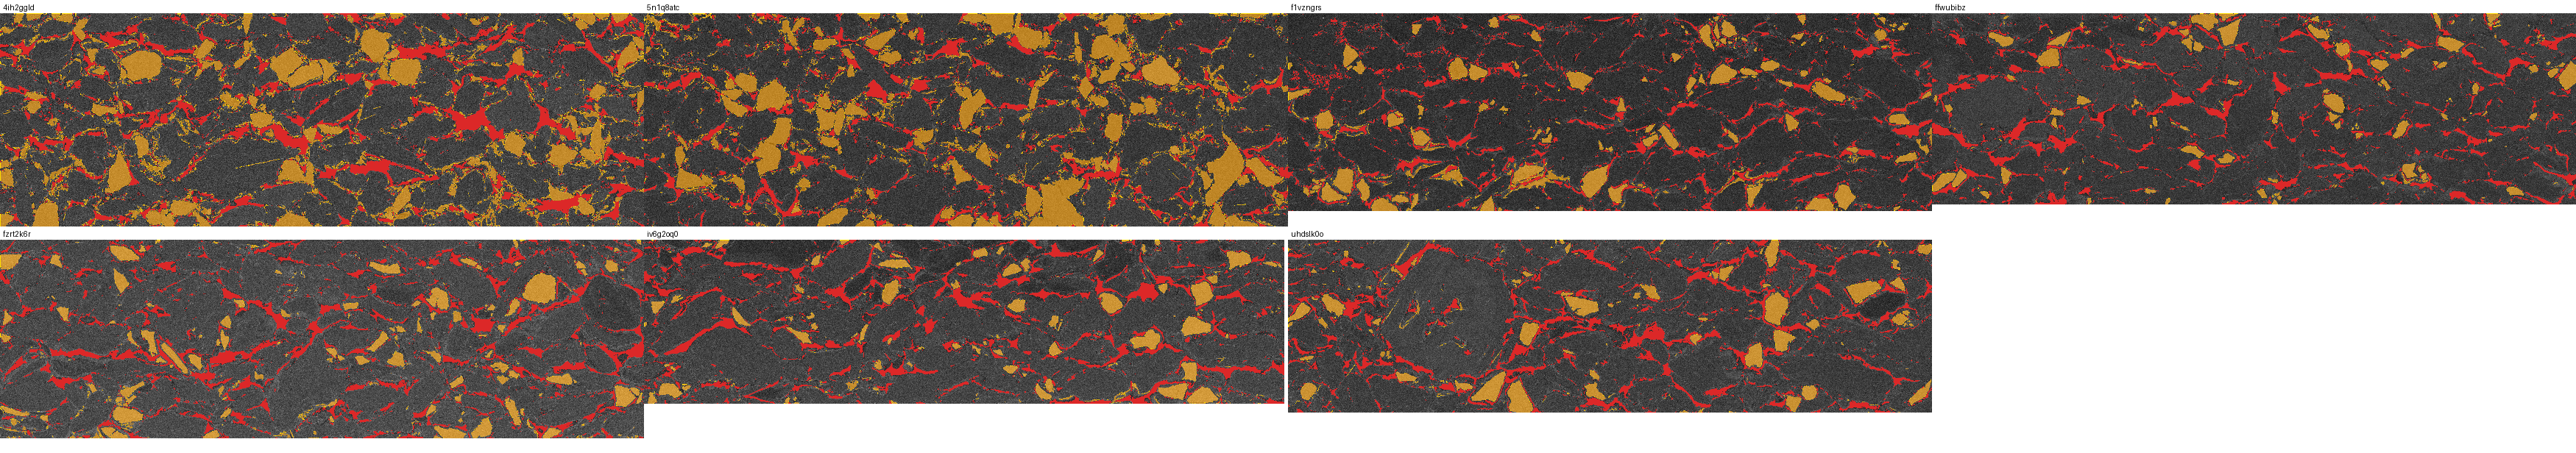
\includegraphics[width=0.95\textwidth]{../overlays/contact_Batch_1.png}
\caption{Batch\_1: segmentation contact sheet (pore=blue, silicon=red overlay on BSE).}\label{fig:contactBatch_1}
\end{figure}

\begin{figure}[H]\centering
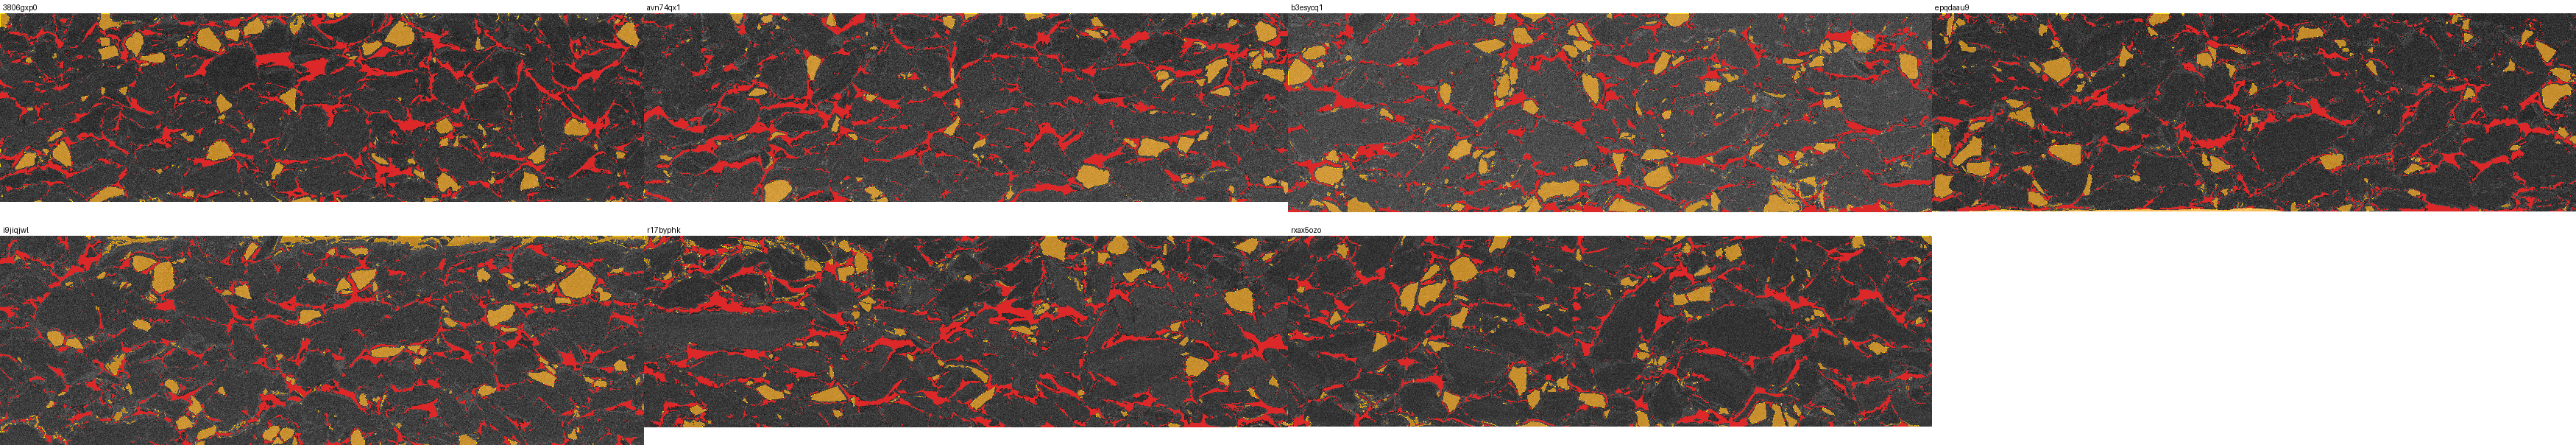
\includegraphics[width=0.95\textwidth]{../overlays/contact_Batch_2.png}
\caption{Batch\_2: segmentation contact sheet (pore=blue, silicon=red overlay on BSE).}\label{fig:contactBatch_2}
\end{figure}

\begin{figure}[H]\centering
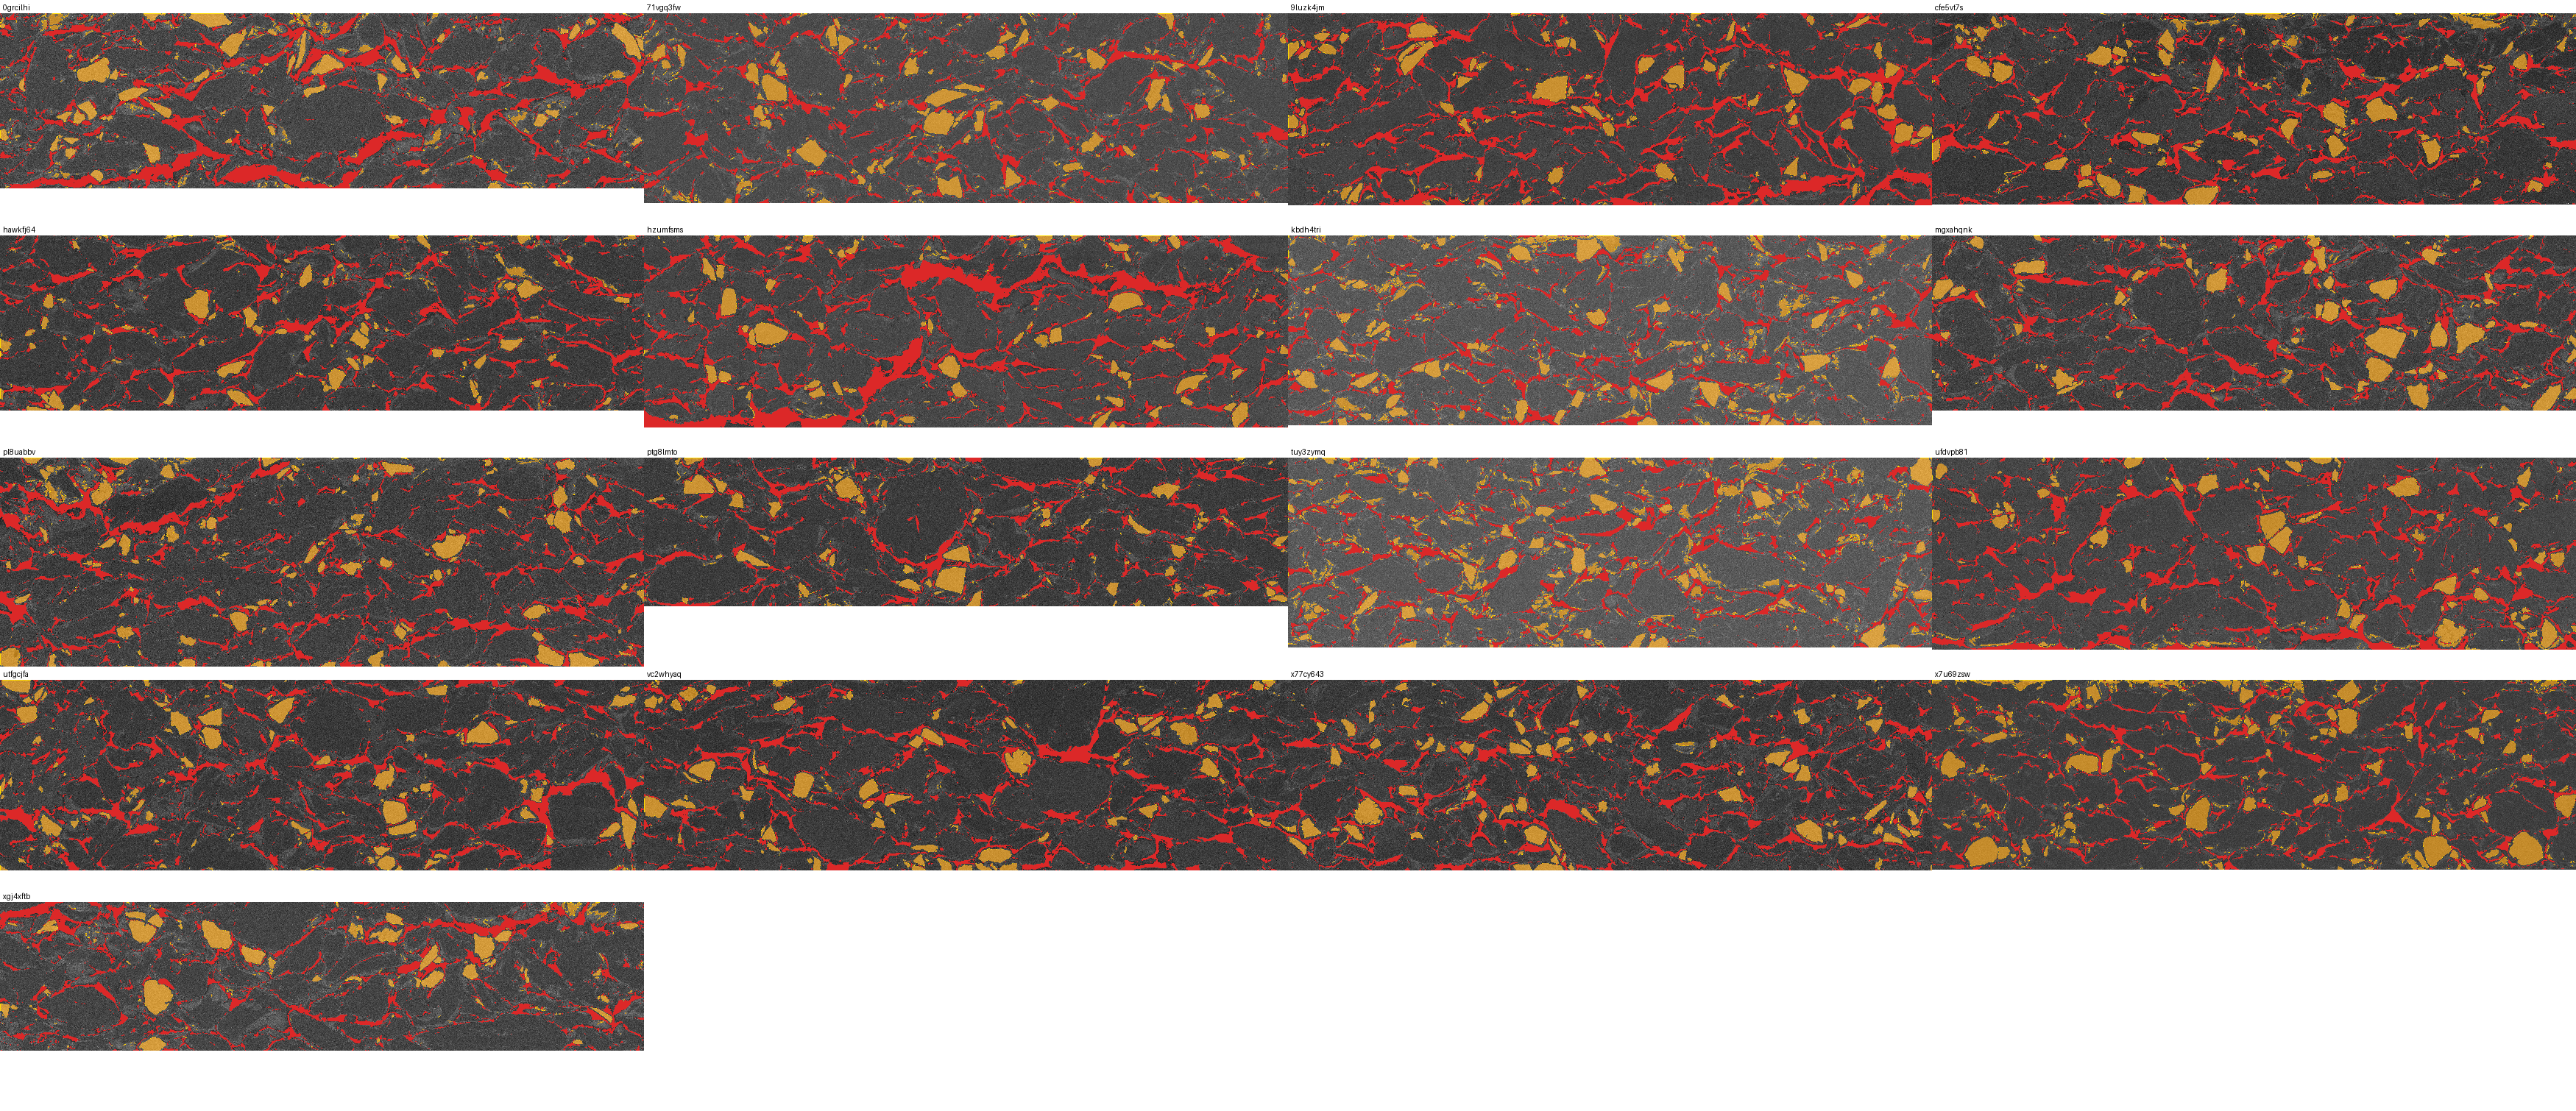
\includegraphics[width=0.95\textwidth]{../overlays/contact_Batch_3.png}
\caption{Batch\_3: segmentation contact sheet (pore=blue, silicon=red overlay on BSE).}\label{fig:contactBatch_3}
\end{figure}

\begin{figure}[H]\centering
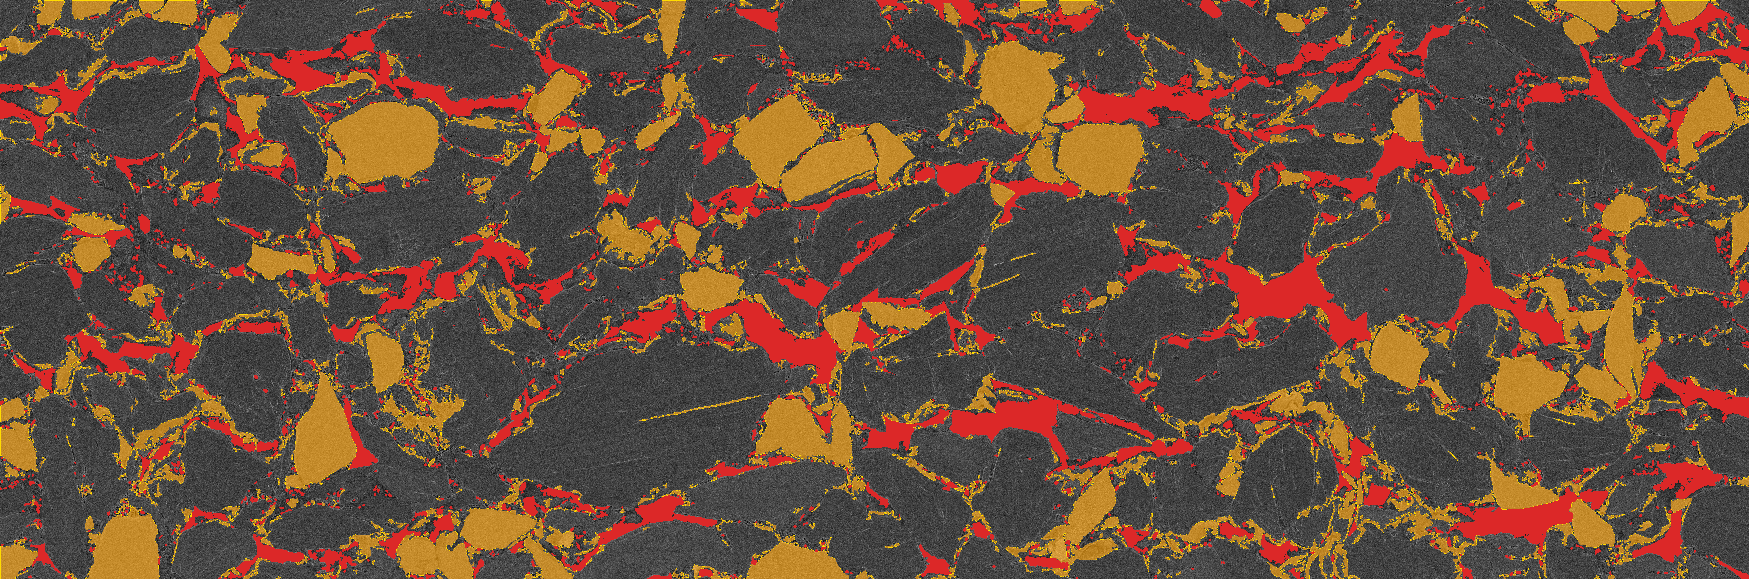
\includegraphics[width=0.95\textwidth]{../overlays/overlay_Batch_1_4ih2ggld.png}
\caption{Flagged image Batch\_1/4ih2ggld overlay.}\label{fig:ovl4ih2ggld}
\end{figure}

\begin{figure}[H]\centering
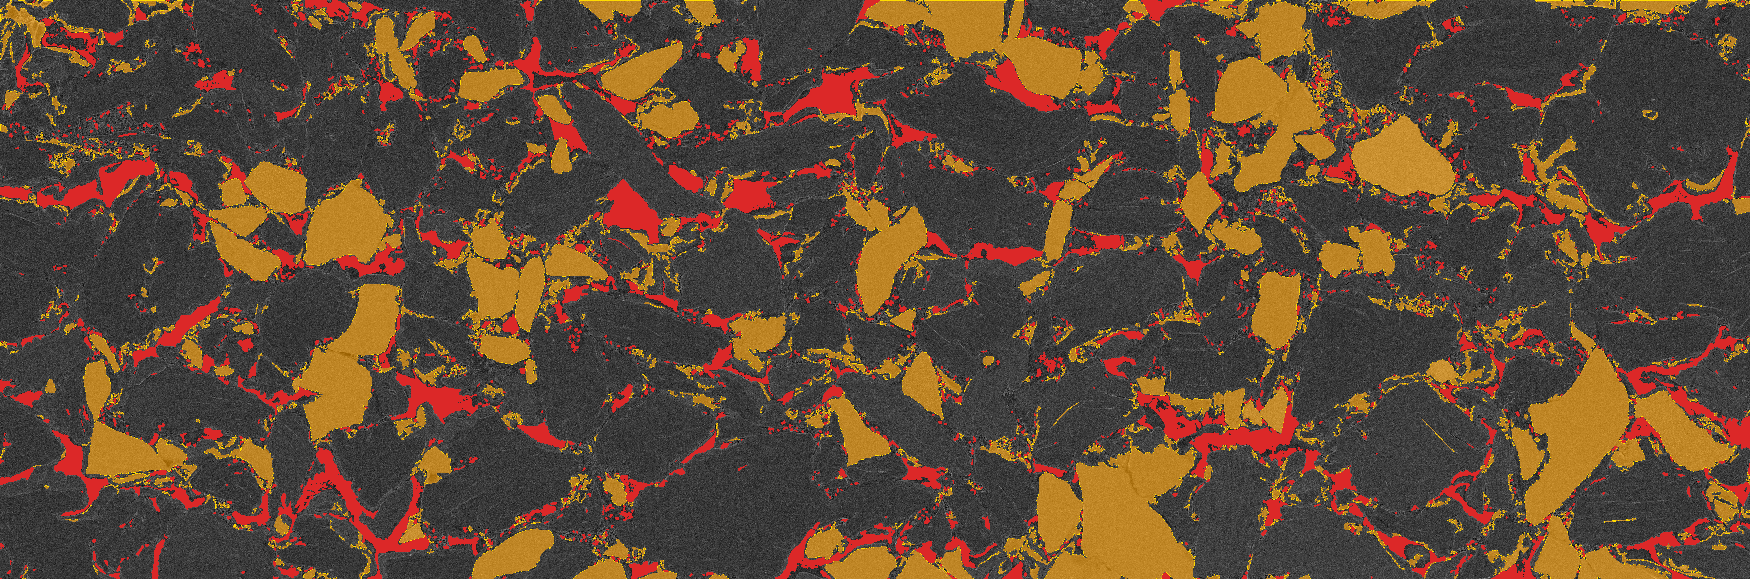
\includegraphics[width=0.95\textwidth]{../overlays/overlay_Batch_1_5n1q8atc.png}
\caption{Flagged image Batch\_1/5n1q8atc overlay.}\label{fig:ovl5n1q8atc}
\end{figure}

\newpage


\section{Phase 2 --- Feature dictionary}
Every feature is explainable in one sentence; references were actually opened
(citations in \texttt{features.xlsx}, FeatureDict sheet). Retained after
pruning (constant, left/right corr $<$0.5, or duplicate $|$r$|>$0.9):
\scriptsize
\begin{longtable}{llllp{4.6cm}p{4.2cm}r}
\caption{Retained features with left/right repeatability}\label{tab:featdict}\\
\toprule
\textbf{feature} & \textbf{group} & \textbf{units} & \textbf{detector} & \textbf{definition} & \textbf{meaning} & \textbf{lr\_corr} \\
\midrule
\endfirsthead
\toprule \textbf{feature} & \textbf{group} & \textbf{units} & \textbf{detector} & \textbf{definition} & \textbf{meaning} & \textbf{lr\_corr} \\
\midrule
\endhead
\midrule\multicolumn{7}{r}{\footnotesize cont.}\\\midrule\endfoot
\bottomrule\endlastfoot
pore\_frac & composition & 1 & BSE & Area fraction of the pore/crack class. & Visible pore volume proxy; lower porosity follows heavier calendering. & 0.8721 \\
graphite\_frac & composition & 1 & BSE & Area fraction of the grey bulk class. & Assumed-graphite share of the section. & 0.6955 \\
silicon\_frac & composition & 1 & BSE & Area fraction of the bright-particle class. & Assumed-silicon share of the section. & 0.7413 \\
si\_d50\_um & silicon & um & BSE & Median number-weighted equivalent diameter. & Typical Si particle size. & 0.6995 \\
si\_solidity & silicon & 1 & BSE & Area-weighted mean solidity (area / convex-hull area) of particles. & Particle angularity / surface regularity. & 0.6016 \\
gr\_chord\_h\_um & graphite & um & BSE & Mean horizontal uninterrupted chord through the graphite phase. & Graphite flake lateral extent proxy. & 0.7319 \\
gr\_chord\_ratio\_hv & graphite & 1 & BSE & gr\_chord\_h\_um / gr\_chord\_v\_um. & Flake alignment: >1 means flakes wider than tall (calendering signature). & 0.6076 \\
gr\_st\_coherence & graphite & 1 & BSE & Structure-tensor coherence of the BSE gradient inside graphite (sigma=5 px). & Local orientation order of the graphite texture. & 0.953 \\
pore\_thick\_d10\_um & pores & um & BSE & 10th percentile of pore local thickness (2x distance transform). & Fine end of the pore-size distribution. & 0.525 \\
pore\_thick\_d50\_um & pores & um & BSE & Median pore local thickness. & Typical pore size. & 0.5828 \\
large\_gap\_frac & pores & 1 & BSE & Area share of pores occupying >0.5\% of the image each. & Large gaps / pull-outs between grains. & 0.7261 \\
pores\_per\_mm2 & pores & mm\textasciicircum -2 & BSE & Number of discrete pore objects per mm\textasciicircum 2. & Pore number density. & 0.6297 \\
ring\_porosity\_250nm & si\_pore & 1 & BSE & Pore fraction in the 10 px (\textasciitilde 250 nm) ring around all Si particles. & Void space immediately adjacent to Si - expansion room. & 0.684 \\
ring\_porosity\_500nm & si\_pore & 1 & BSE & Pore fraction in the 10-20 px (\textasciitilde 250-500 nm) ring around all Si particles. & Void space in the near neighbourhood of Si. & 0.62 \\
corr\_len\_gr\_um & spatial & um & BSE & Same for the graphite phase. & Graphite correlation length. & 0.5288 \\
si\_clarkevans\_R & spatial & 1 & BSE & Observed/expected nearest-centroid distance vs random, Donnelly edge correction. & <1 clustered, \textasciitilde 1 random, >1 ordered Si dispersion. & 0.5947 \\
inlens\_edge\_density & texture & 1 & Inlens & Mean gradient magnitude of the Inlens image (normalised units/px). & Surface fine-crack / edge density. & 0.962 \\
inlens\_bulk\_texture & texture & 1 & Inlens & Std of Inlens grey level inside the graphite class. & Surface texture roughness of the bulk. & 0.9296 \\
etd\_roughness & texture & 1 & ETD & RMS gradient magnitude of the ETD/SE topography image. & Topographic roughness proxy. & 0.9638 \\
bse\_bulk\_texture & texture & 1 & BSE & Std of BSE grey level inside the graphite class. & Compositional micro-texture of the graphite. & 0.9839 \\
\end{longtable}
\normalsize
\scriptsize
\begin{longtable}{lp{10cm}}
\caption{Dropped features and why}\label{tab:dropped}\\
\toprule
\textbf{feature} & \textbf{reason} \\
\midrule
\endfirsthead
\toprule \textbf{feature} & \textbf{reason} \\
\midrule
\endhead
\midrule\multicolumn{2}{r}{\footnotesize cont.}\\\midrule\endfoot
\bottomrule\endlastfoot
si\_share\_of\_solid & duplicate of silicon\_frac (|r|>0.9) \\
si\_per\_mm2 & duplicate of silicon\_frac (|r|>0.9) \\
si\_d90\_um & left/right corr 0.19 < 0.5 \\
si\_d99\_um & left/right corr -0.10 < 0.5 \\
si\_dmax\_um & left/right corr 0.01 < 0.5 \\
si\_d50\_area\_um & left/right corr 0.08 < 0.5 \\
si\_large\_area\_frac & left/right corr 0.20 < 0.5 \\
si\_aspect & left/right corr -0.00 < 0.5 \\
si\_sv & left/right corr 0.42 < 0.5 \\
si\_cracked\_share & left/right corr nan (unrepeatable: one/both halves constant) \\
gr\_chord\_v\_um & duplicate of gr\_chord\_h\_um (|r|>0.9) \\
gr\_sv & left/right corr 0.36 < 0.5 \\
pore\_thick\_d90\_um & duplicate of pore\_thick\_d50\_um (|r|>0.9) \\
crack\_frac & left/right corr 0.26 < 0.5 \\
compact\_pore\_frac & left/right corr 0.21 < 0.5 \\
pore\_chord\_h\_um & duplicate of pore\_frac (|r|>0.9) \\
pore\_chord\_v\_um & duplicate of pore\_frac (|r|>0.9) \\
pore\_anisotropy & left/right corr 0.48 < 0.5 \\
pore\_depth\_cv & left/right corr -0.05 < 0.5 \\
pore\_depth\_slope & left/right corr 0.08 < 0.5 \\
crack\_len\_density & left/right corr 0.47 < 0.5 \\
si\_pore\_dist\_mean\_um & left/right corr 0.16 < 0.5 \\
si\_no\_pore\_share & left/right corr 0.34 < 0.5 \\
corr\_len\_pore\_um & duplicate of pore\_thick\_d50\_um (|r|>0.9) \\
corr\_len\_si\_um & left/right corr 0.02 < 0.5 \\
lineal\_path\_pore\_um & duplicate of pore\_frac (|r|>0.9) \\
pore\_patchiness\_cv & left/right corr 0.33 < 0.5 \\
si\_patchiness\_cv & left/right corr 0.27 < 0.5 \\
tau\_x & left/right corr nan (unrepeatable: one/both halves constant) \\
tau\_y & left/right corr nan (unrepeatable: one/both halves constant) \\
pore\_percolates\_x & constant or >50\% missing \\
pore\_percolates\_y & constant or >50\% missing \\
pore\_largest\_cc\_frac & duplicate of large\_gap\_frac (|r|>0.9) \\
\end{longtable}
\normalsize
\newpage


\section{Phase 3 --- Batch\_3 baseline}
Statistics over 17 images; bootstrap CI on the mean (2{,}000 resamples);
envelope = 5th--95th percentile. Internal consistency uses robust z-scores
(median/MAD) per feature.
\scriptsize
\begin{longtable}{lrrrrrrr}
\caption{Batch\_3 baseline statistics}\label{tab:baseline}\\
\toprule
\textbf{feature} & \textbf{mean} & \textbf{median} & \textbf{std} & \textbf{p5} & \textbf{p95} & \textbf{ci95\_lo} & \textbf{ci95\_hi} \\
\midrule
\endfirsthead
\toprule \textbf{feature} & \textbf{mean} & \textbf{median} & \textbf{std} & \textbf{p5} & \textbf{p95} & \textbf{ci95\_lo} & \textbf{ci95\_hi} \\
\midrule
\endhead
\midrule\multicolumn{8}{r}{\footnotesize cont.}\\\midrule\endfoot
\bottomrule\endlastfoot
pore\_frac & 0.1142 & 0.108 & 0.0217 & 0.0927 & 0.1537 & 0.1054 & 0.1248 \\
graphite\_frac & 0.819 & 0.8218 & 0.0192 & 0.7856 & 0.8473 & 0.8098 & 0.8275 \\
silicon\_frac & 0.0668 & 0.0611 & 0.014 & 0.0499 & 0.0937 & 0.0609 & 0.0731 \\
si\_d50\_um & 0.763 & 0.6852 & 0.2052 & 0.5653 & 1.123 & 0.6763 & 0.8627 \\
si\_solidity & 0.8959 & 0.8981 & 0.0177 & 0.8635 & 0.9128 & 0.8876 & 0.903 \\
gr\_chord\_h\_um & 3.668 & 3.717 & 0.4279 & 2.966 & 4.236 & 3.471 & 3.856 \\
gr\_chord\_ratio\_hv & 1.2 & 1.192 & 0.0378 & 1.151 & 1.263 & 1.183 & 1.217 \\
gr\_st\_coherence & 0.1084 & 0.11 & 0.0081 & 0.0939 & 0.1181 & 0.1045 & 0.1118 \\
pore\_thick\_d10\_um & 0.0537 & 0.05 & 0.0081 & 0.05 & 0.0707 & 0.05 & 0.0573 \\
pore\_thick\_d50\_um & 0.2697 & 0.25 & 0.046 & 0.2213 & 0.3674 & 0.2511 & 0.2921 \\
large\_gap\_frac & 0.0148 & 0.0085 & 0.0202 & 0 & 0.0599 & 0.0069 & 0.0247 \\
pores\_per\_mm2 & 154,974.6 & 155,027.6 & 12,984.1 & 137,136.5 & 172,640.2 & 148,861.8 & 160,655.5 \\
ring\_porosity\_250nm & 0.0836 & 0.0829 & 0.0216 & 0.0594 & 0.1163 & 0.0746 & 0.0939 \\
ring\_porosity\_500nm & 0.2 & 0.189 & 0.0407 & 0.1583 & 0.2659 & 0.1837 & 0.2188 \\
corr\_len\_gr\_um & 0.9353 & 0.95 & 0.1042 & 0.75 & 1.06 & 0.8882 & 0.9824 \\
si\_clarkevans\_R & 0.6793 & 0.6758 & 0.0434 & 0.6133 & 0.7364 & 0.6599 & 0.6978 \\
inlens\_edge\_density & 0.0402 & 0.042 & 0.0075 & 0.0297 & 0.0496 & 0.0367 & 0.0434 \\
inlens\_bulk\_texture & 50.933 & 50.907 & 11.246 & 38.207 & 64.906 & 45.651 & 56.337 \\
etd\_roughness & 0.0303 & 0.0297 & 0.0035 & 0.026 & 0.0346 & 0.0287 & 0.0319 \\
bse\_bulk\_texture & 11.816 & 12.775 & 1.728 & 9.66 & 13.696 & 10.998 & 12.598 \\
\end{longtable}
\normalsize
Batch\_3 outlier images (robust z $>$3.5 on at least one feature): 0grcilhi, 9luzk4jm, hzumfsms, kbdh4tri, tuy3zymq, x77cy643, x7u69zsw. These are within-batch scatter, not exclusions.

\begin{figure}[H]\centering
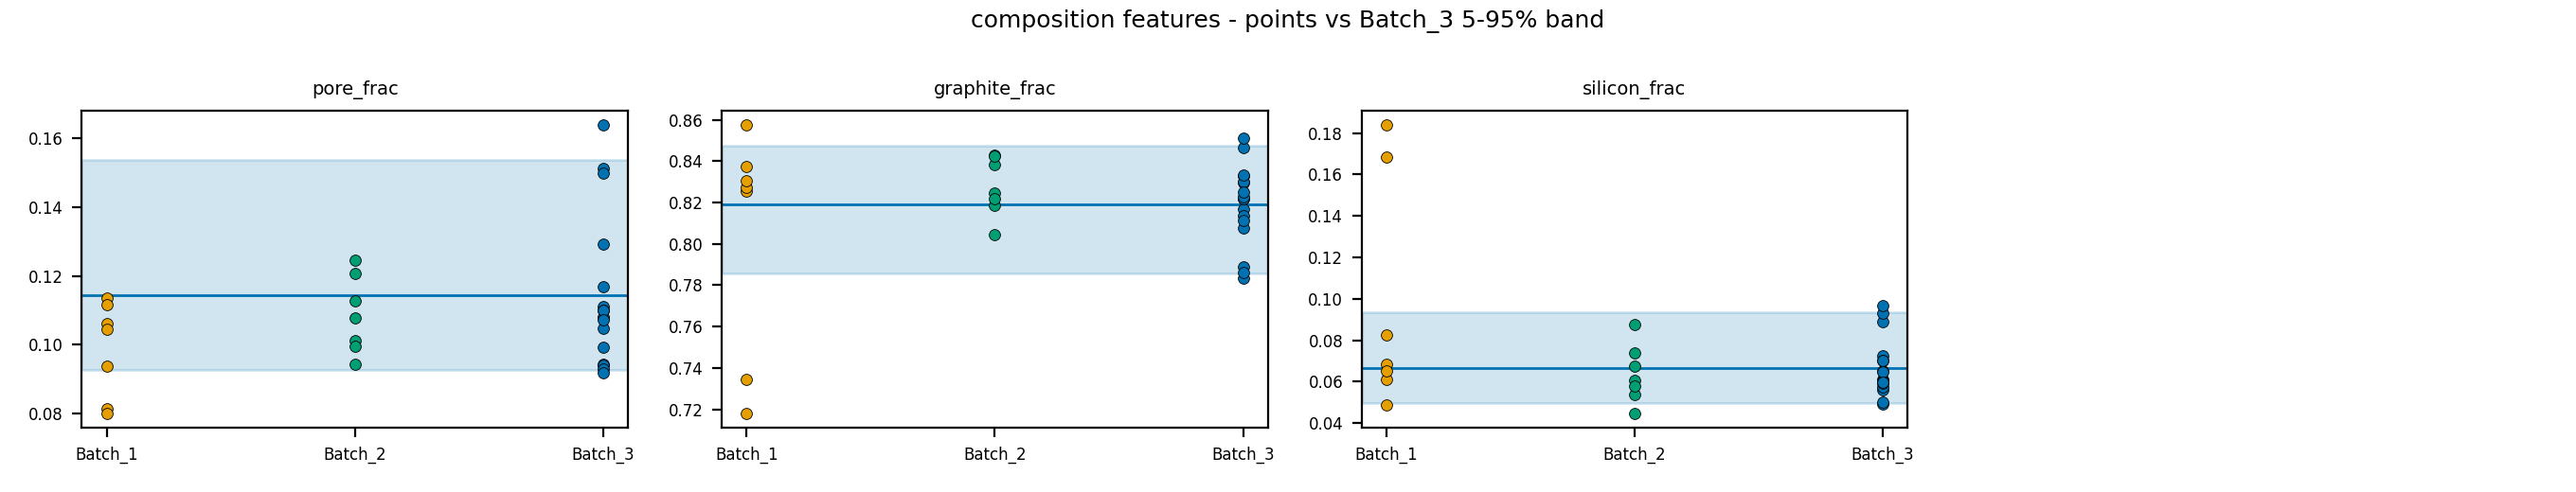
\includegraphics[width=0.95\textwidth]{../figures/features_composition.png}
\caption{composition --- every image as a point against the Batch\_3 5--95\% band.}\label{fig:features_composition}
\end{figure}

\begin{figure}[H]\centering
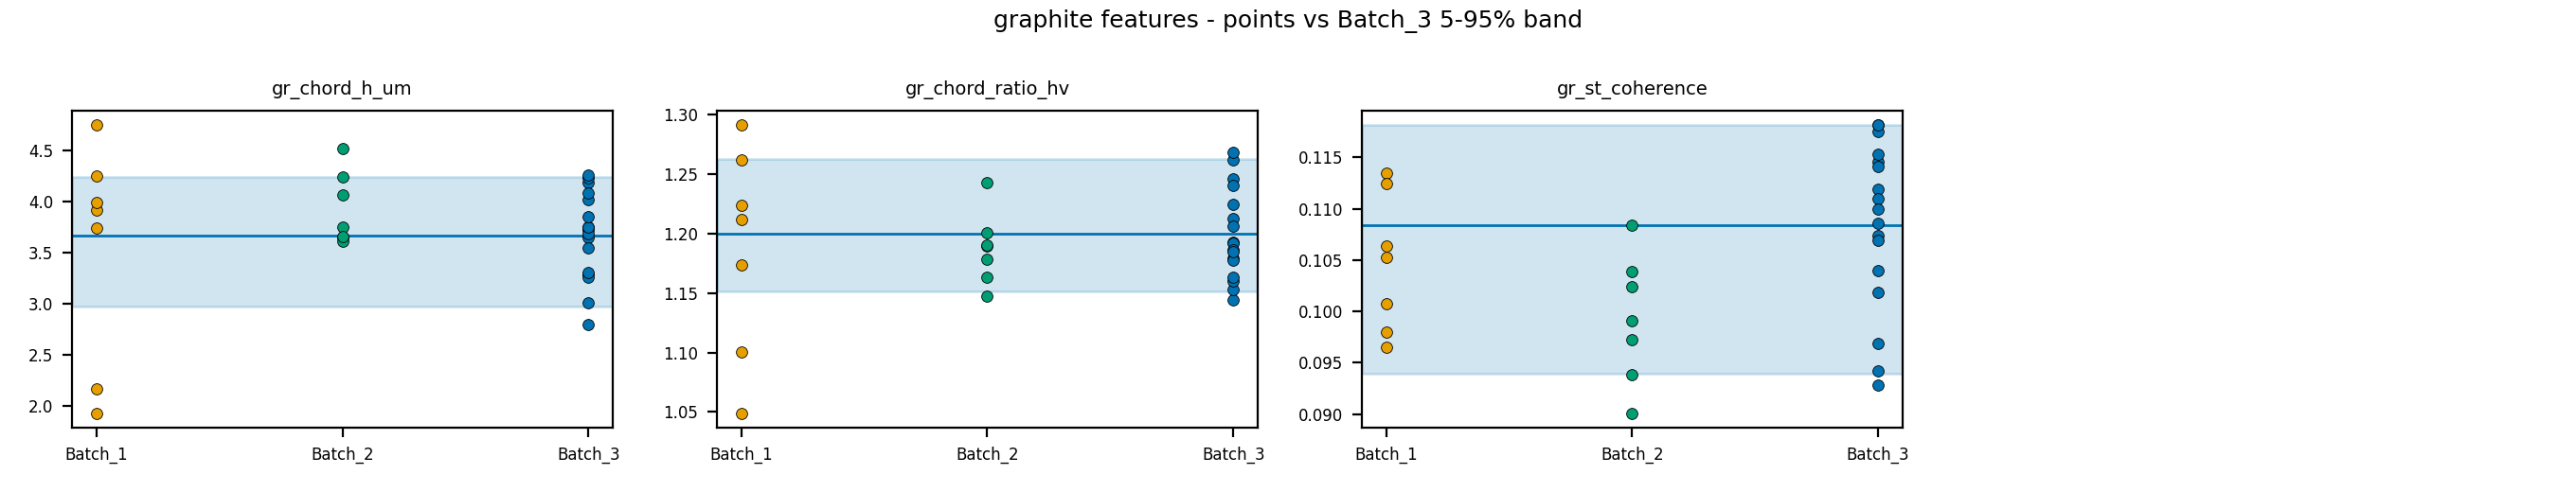
\includegraphics[width=0.95\textwidth]{../figures/features_graphite.png}
\caption{graphite --- every image as a point against the Batch\_3 5--95\% band.}\label{fig:features_graphite}
\end{figure}

\begin{figure}[H]\centering
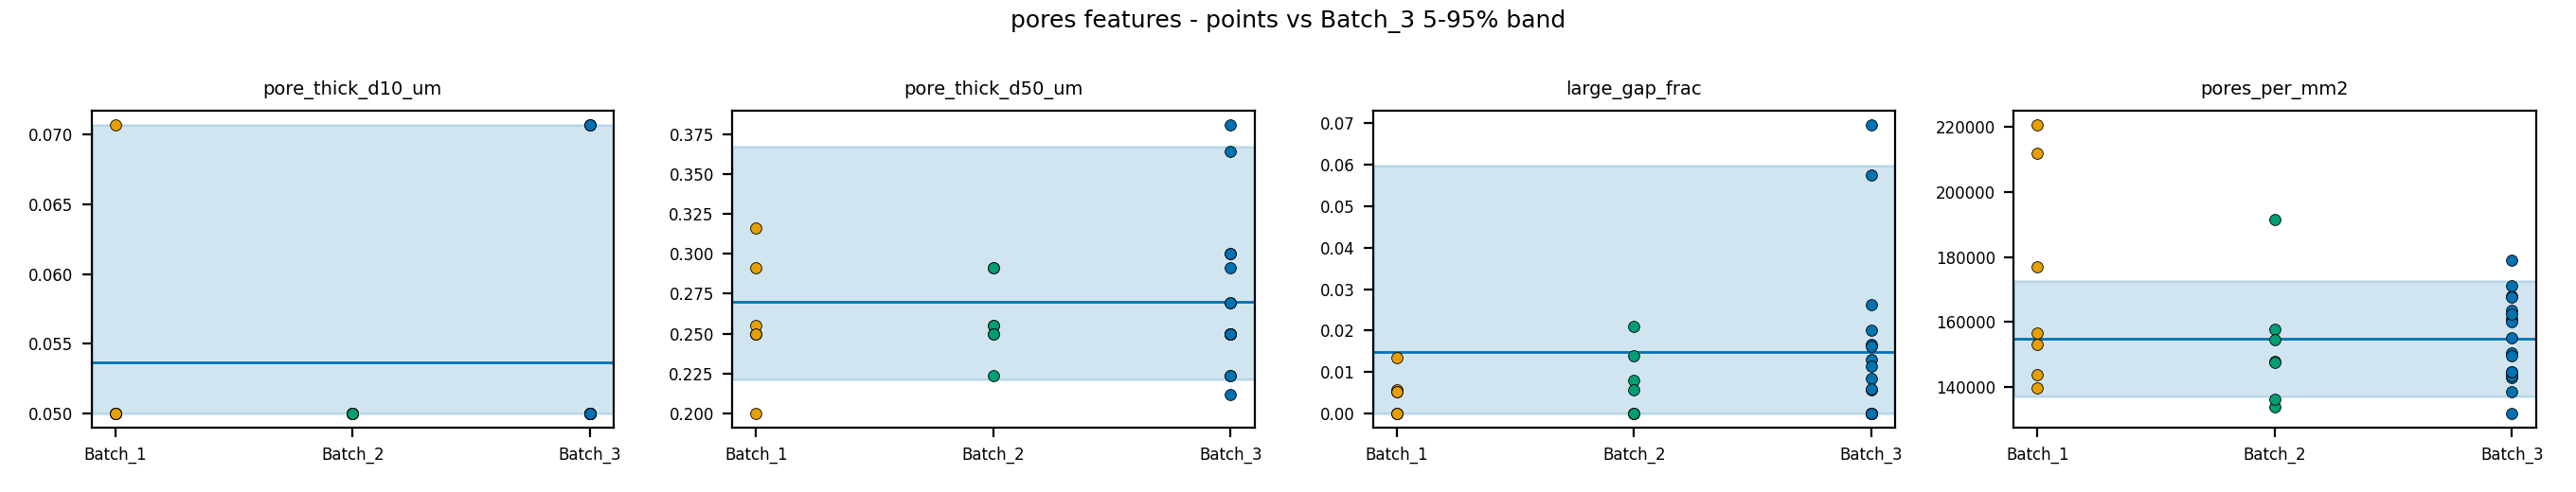
\includegraphics[width=0.95\textwidth]{../figures/features_pores.png}
\caption{pores --- every image as a point against the Batch\_3 5--95\% band.}\label{fig:features_pores}
\end{figure}

\begin{figure}[H]\centering
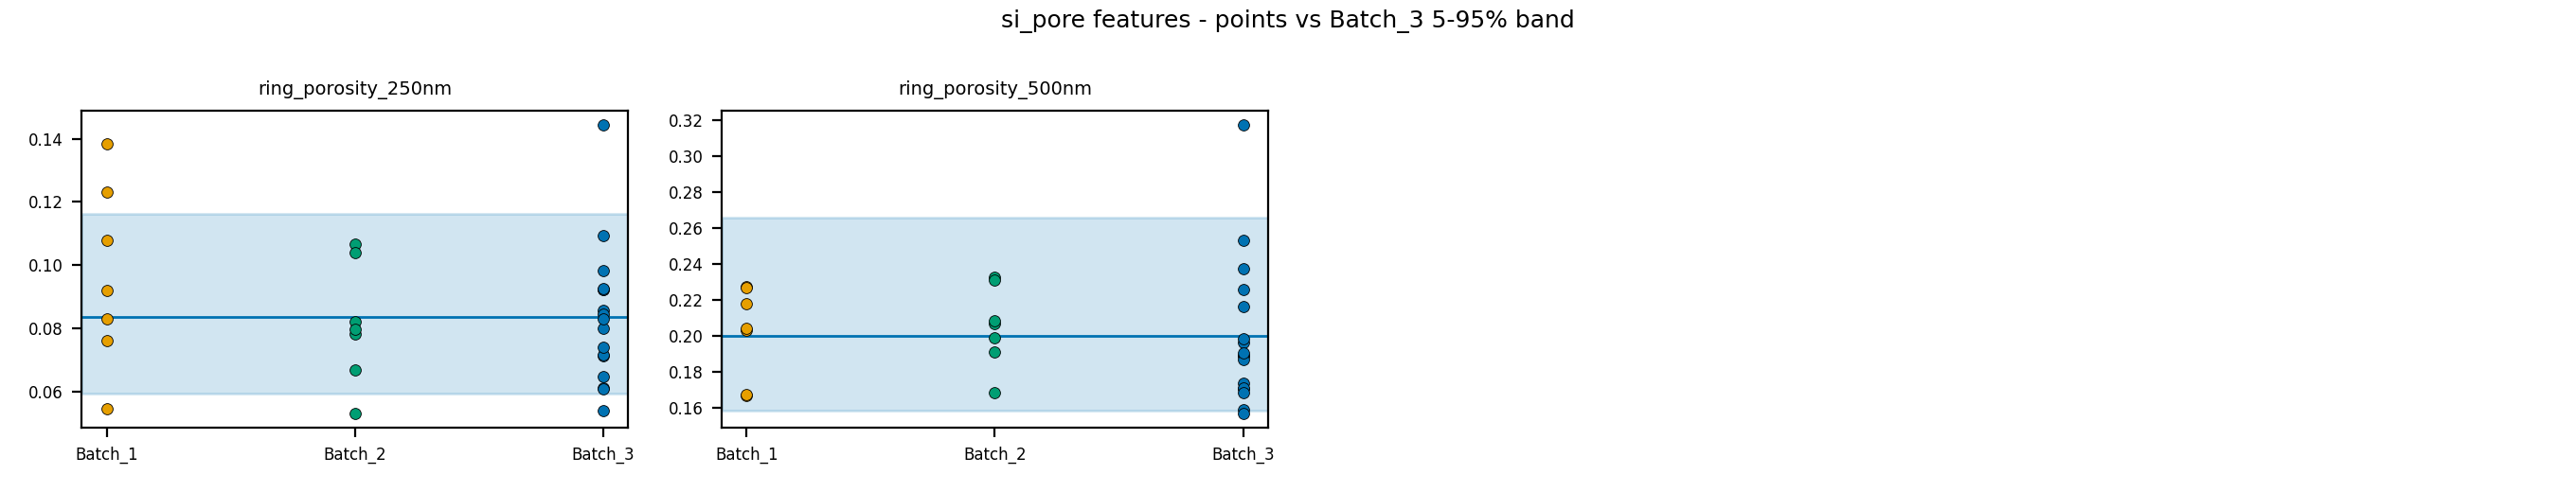
\includegraphics[width=0.95\textwidth]{../figures/features_si_pore.png}
\caption{si pore --- every image as a point against the Batch\_3 5--95\% band.}\label{fig:features_si_pore}
\end{figure}

\begin{figure}[H]\centering
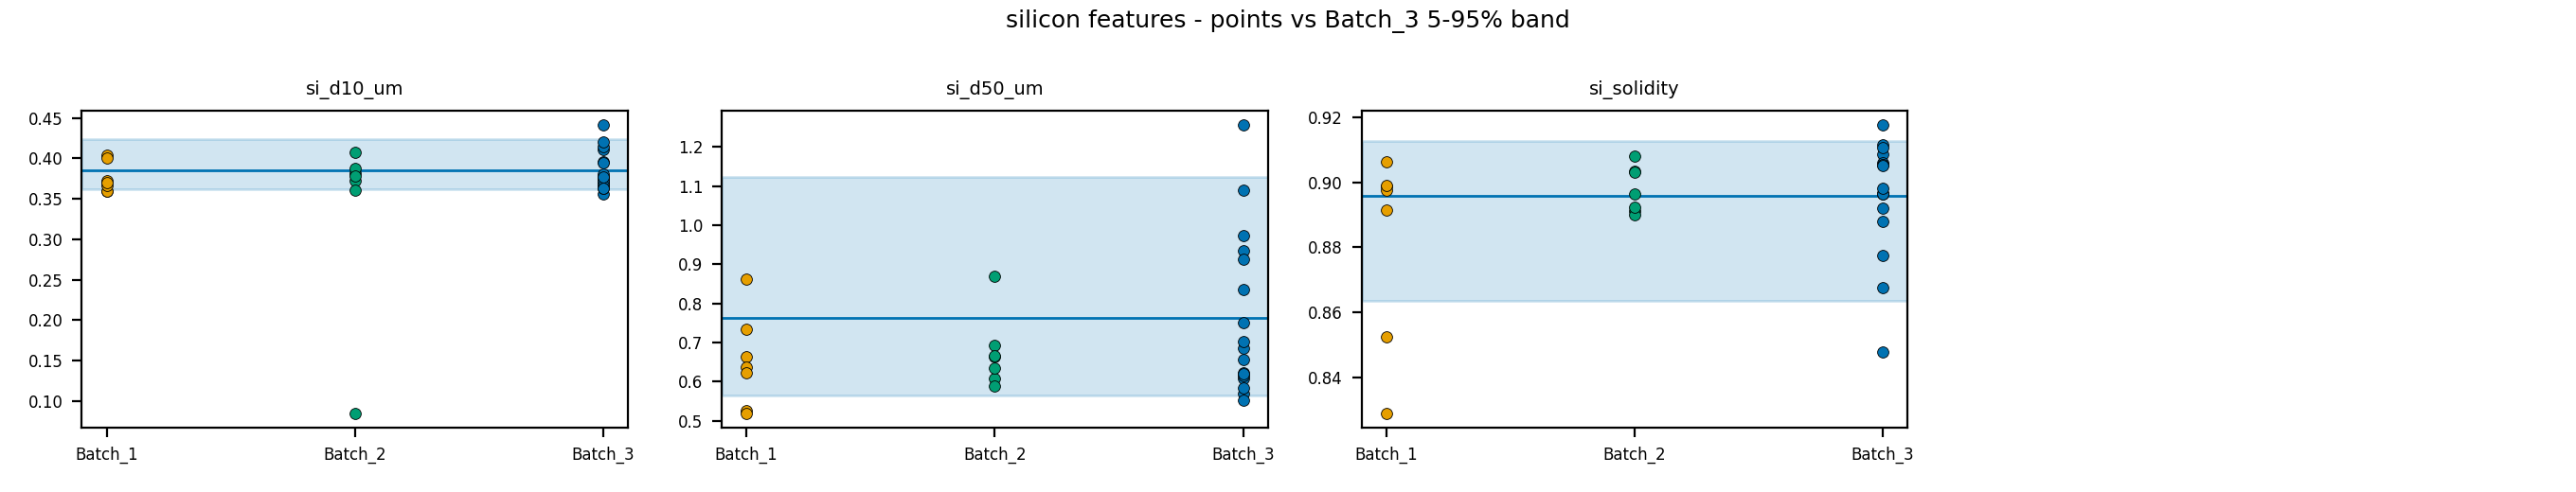
\includegraphics[width=0.95\textwidth]{../figures/features_silicon.png}
\caption{silicon --- every image as a point against the Batch\_3 5--95\% band.}\label{fig:features_silicon}
\end{figure}

\begin{figure}[H]\centering
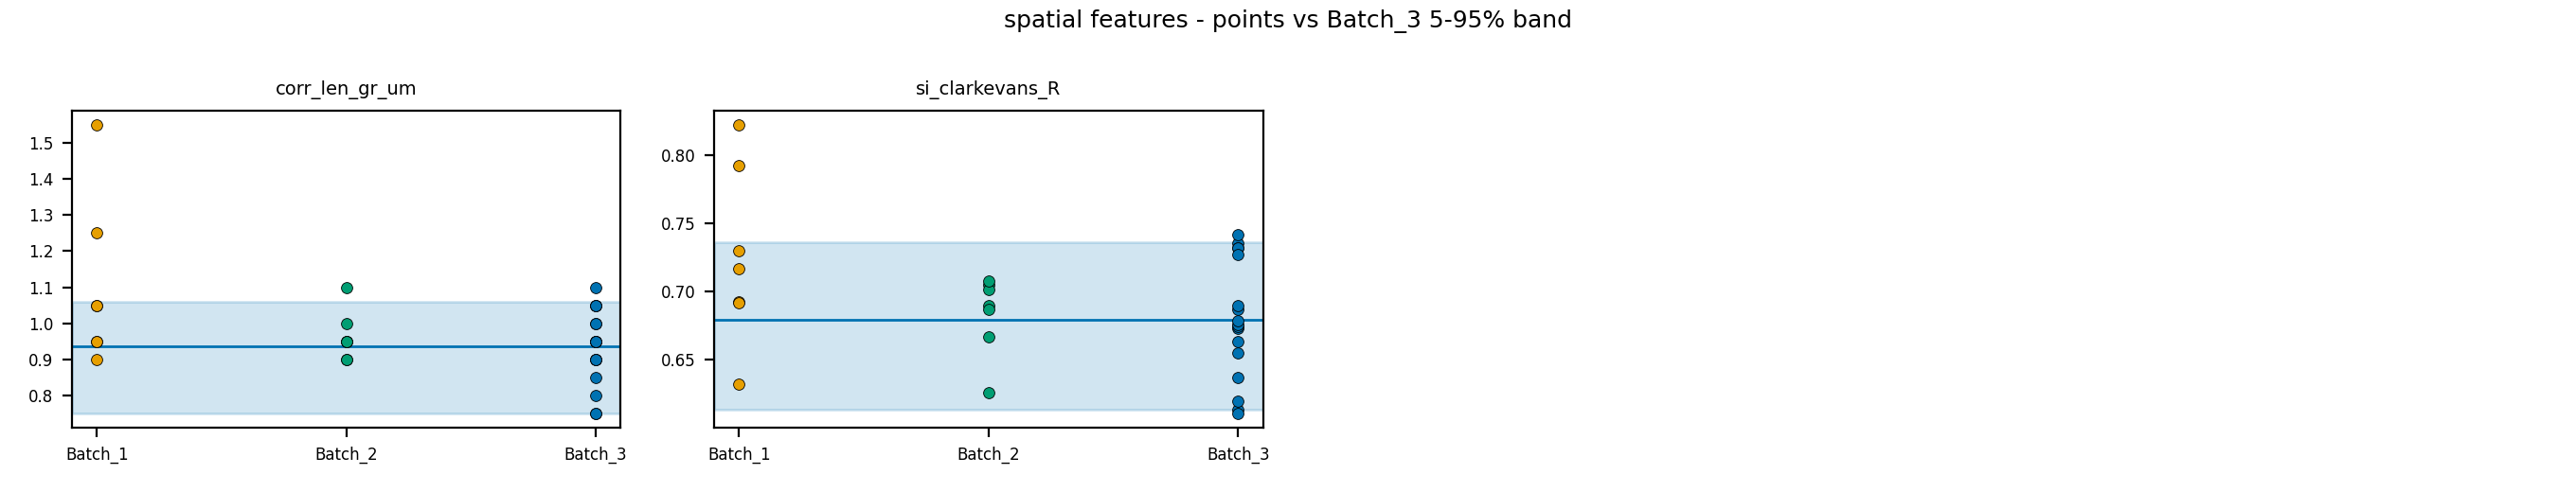
\includegraphics[width=0.95\textwidth]{../figures/features_spatial.png}
\caption{spatial --- every image as a point against the Batch\_3 5--95\% band.}\label{fig:features_spatial}
\end{figure}

\begin{figure}[H]\centering
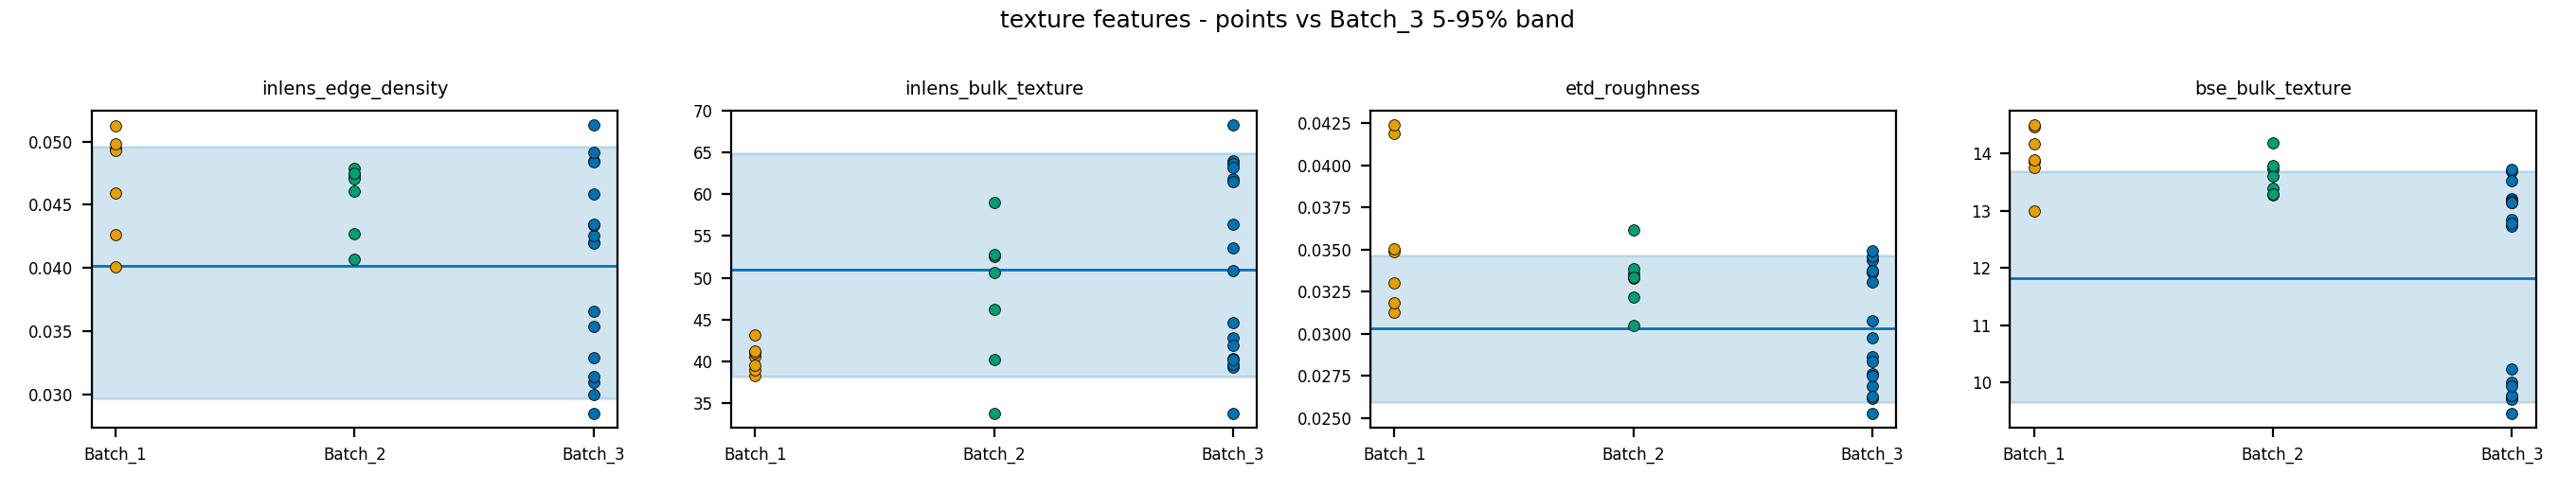
\includegraphics[width=0.95\textwidth]{../figures/features_texture.png}
\caption{texture --- every image as a point against the Batch\_3 5--95\% band.}\label{fig:features_texture}
\end{figure}

\begin{figure}[H]\centering
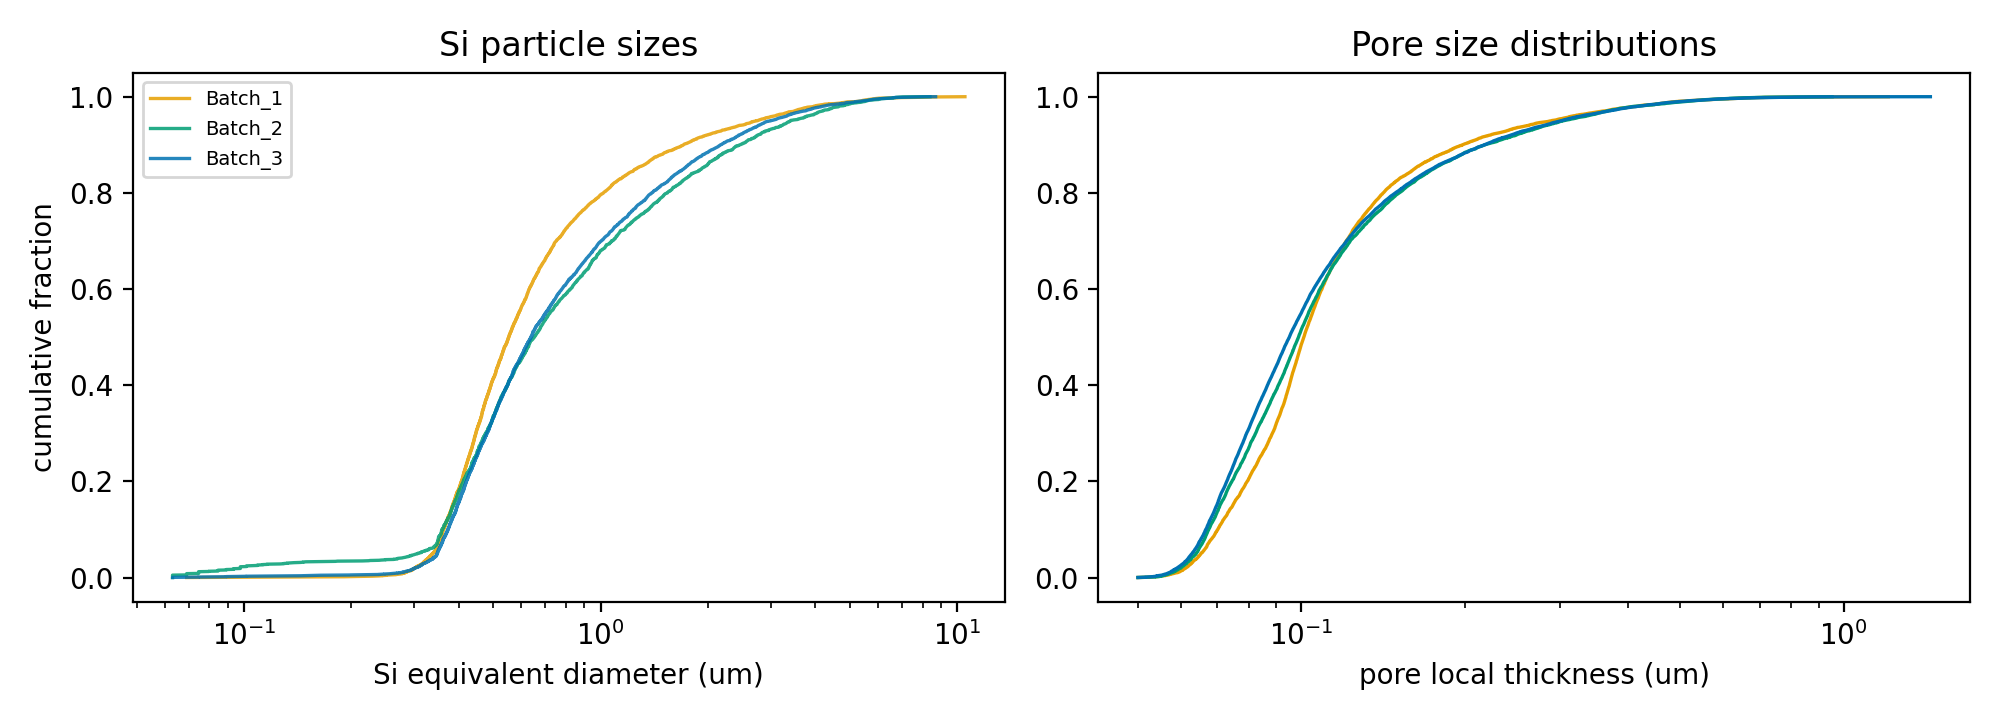
\includegraphics[width=0.95\textwidth]{../figures/distributions.png}
\caption{Size and pore distributions overlaid per batch.}\label{fig:dists}
\end{figure}

\begin{figure}[H]\centering
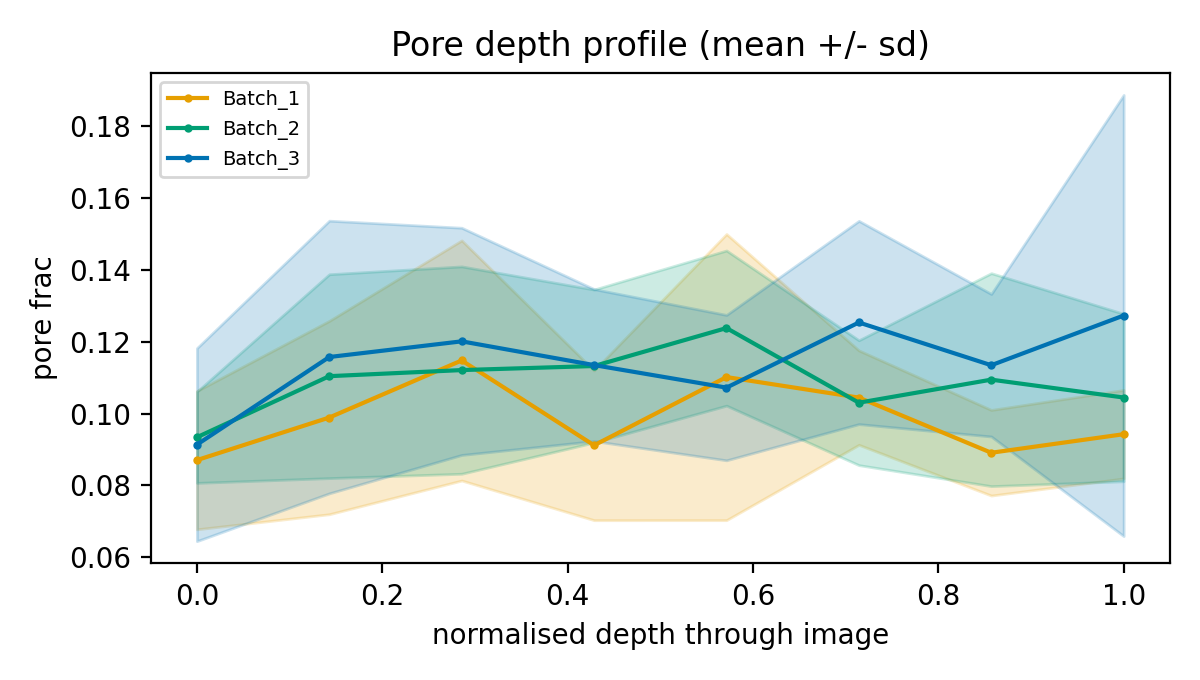
\includegraphics[width=0.95\textwidth]{../figures/pore_depth.png}
\caption{Pore fraction depth profile across the field of view.}\label{fig:depth}
\end{figure}

\newpage


\section{Phase 4 --- DFN simulation}
PyBaMM \texttt{BasicDFNComposite} + published \texttt{Chen2020\_composite}
(LGM50 NMC811 / graphite-SiO$_x$). Image-derived inputs per batch below;
everything else at published values and identical for all batches.
Uncertainty bands resample the image-derived inputs (30 draws). Porosity is
run twice: the measured visible value \emph{and} corrected to 0.30
(literature range for calendered anodes), because pores below the
$\sim$50~nm pixel size are unresolved. Absolute values are NOT validated ---
only batch-to-batch differences are meaningful; the model includes no
swelling, cracking or ageing.
\scriptsize
\begin{longtable}{lrrrrr}
\caption{Image-derived DFN inputs (batch means)}\label{tab:dfninputs}\\
\toprule
\textbf{batch} & \textbf{porosity} & \textbf{graphite amf} & \textbf{silicon amf} & \textbf{r\_graphite $\mu$m} & \textbf{r\_Si $\mu$m} \\
\midrule
\endfirsthead
\toprule \textbf{batch} & \textbf{porosity} & \textbf{graphite amf} & \textbf{silicon amf} & \textbf{r\_graphite $\mu$m} & \textbf{r\_Si $\mu$m} \\
\midrule
\endhead
\midrule\multicolumn{6}{r}{\footnotesize cont.}\\\midrule\endfoot
\bottomrule\endlastfoot
Batch\_1 & 0.0987 & 0.8044 & 0.0969 & 2.648 & 0.326 \\
Batch\_2 & 0.1087 & 0.8276 & 0.0637 & 2.943 & 0.337 \\
Batch\_3 & 0.1142 & 0.819 & 0.0668 & 2.751 & 0.382 \\
\end{longtable}
\normalsize
\scriptsize
\begin{longtable}{lp{5cm}p{5.5cm}}
\caption{DFN assumptions}\label{tab:dfnass}\\
\toprule
\textbf{parameter} & \textbf{value} & \textbf{note} \\
\midrule
\endfirsthead
\toprule \textbf{parameter} & \textbf{value} & \textbf{note} \\
\midrule
\endhead
\midrule\multicolumn{3}{r}{\footnotesize cont.}\\\midrule\endfoot
\bottomrule\endlastfoot
model & pybamm.lithium\_ion.BasicDFNComposite & composite graphite-SiOx negative, full-cell NMC811 \\
parameter set & Chen2020\_composite (LGM50) & published, unchanged where not image-derived \\
Negative electrode porosity & image value  OR corrected to 0.30 (literature range) & two runs; visible porosity underestimates true \\
active material volume fractions & scaled from image graphite/silicon fractions & primary=graphite, secondary=SiOx \\
particle radii & graphite: 0.75*chord length; silicon: D50/2 & chord->radius conversion documented \\
Negative electrode thickness & 85.2 um (parameter set), swept 60/85.2/110 um & not visible in top-down SEM \\
Bruggeman exponent & 1.5 (parameter set) & kept at published value \\
everything else & Chen2020\_composite defaults & identical for all batches \\
\end{longtable}
\normalsize
\scriptsize
\begin{longtable}{lrrrrrrr}
\caption{Discharge capacity (Ah) per batch / porosity mode / C-rate --- 30 resamples}\label{tab:dfncap}\\
\toprule
\textbf{batch} & \textbf{porosity\_mode} & \textbf{c\_rate} & \textbf{n} & \textbf{cap\_mean} & \textbf{cap\_std} & \textbf{cap\_p5} & \textbf{cap\_p95} \\
\midrule
\endfirsthead
\toprule \textbf{batch} & \textbf{porosity\_mode} & \textbf{c\_rate} & \textbf{n} & \textbf{cap\_mean} & \textbf{cap\_std} & \textbf{cap\_p5} & \textbf{cap\_p95} \\
\midrule
\endhead
\midrule\multicolumn{8}{r}{\footnotesize cont.}\\\midrule\endfoot
\bottomrule\endlastfoot
Batch\_1 & measured & 0.1 & 30 & 5.25 & 0. & 5.25 & 5.25 \\
Batch\_1 & measured & 0.5 & 30 & 5.25 & 0. & 5.25 & 5.25 \\
Batch\_1 & measured & 1 & 30 & 5.25 & 0. & 5.25 & 5.25 \\
Batch\_1 & measured & 2 & 30 & 3.813 & 0.1453 & 3.564 & 4.021 \\
Batch\_1 & corrected & 0.1 & 30 & 5.25 & 0. & 5.25 & 5.25 \\
Batch\_1 & corrected & 0.5 & 30 & 5.25 & 0. & 5.25 & 5.25 \\
Batch\_1 & corrected & 1 & 30 & 5.25 & 0. & 5.25 & 5.25 \\
Batch\_1 & corrected & 2 & 30 & 5.114 & 0.0008 & 5.113 & 5.115 \\
Batch\_2 & measured & 0.1 & 30 & 5.25 & 0. & 5.25 & 5.25 \\
Batch\_2 & measured & 0.5 & 30 & 5.25 & 0. & 5.25 & 5.25 \\
Batch\_2 & measured & 1 & 30 & 5.25 & 0. & 5.25 & 5.25 \\
Batch\_2 & measured & 2 & 30 & 3.806 & 0.1609 & 3.579 & 3.979 \\
Batch\_2 & corrected & 0.1 & 30 & 5.25 & 0. & 5.25 & 5.25 \\
Batch\_2 & corrected & 0.5 & 30 & 5.25 & 0. & 5.25 & 5.25 \\
Batch\_2 & corrected & 1 & 30 & 5.25 & 0. & 5.25 & 5.25 \\
Batch\_2 & corrected & 2 & 30 & 5.114 & 0.0007 & 5.112 & 5.114 \\
Batch\_3 & measured & 0.1 & 30 & 5.25 & 0. & 5.25 & 5.25 \\
Batch\_3 & measured & 0.5 & 30 & 5.25 & 0. & 5.25 & 5.25 \\
Batch\_3 & measured & 1 & 30 & 5.25 & 0. & 5.25 & 5.25 \\
Batch\_3 & measured & 2 & 30 & 3.92 & 0.1654 & 3.641 & 4.155 \\
Batch\_3 & corrected & 0.1 & 30 & 5.25 & 0. & 5.25 & 5.25 \\
Batch\_3 & corrected & 0.5 & 30 & 5.25 & 0. & 5.25 & 5.25 \\
Batch\_3 & corrected & 1 & 30 & 5.25 & 0. & 5.25 & 5.25 \\
Batch\_3 & corrected & 2 & 30 & 5.114 & 0.0004 & 5.113 & 5.114 \\
\end{longtable}
\normalsize
\scriptsize
\begin{longtable}{lrrrrrrr}
\caption{DFN output deltas vs Batch\_3 (bootstrap CI)}\label{tab:dfndeltas}\\
\toprule
\textbf{batch} & \textbf{porosity\_mode} & \textbf{c\_rate} & \textbf{delta\_ah} & \textbf{pct\_delta} & \textbf{ci\_lo} & \textbf{ci\_hi} & \textbf{sig} \\
\midrule
\endfirsthead
\toprule \textbf{batch} & \textbf{porosity\_mode} & \textbf{c\_rate} & \textbf{delta\_ah} & \textbf{pct\_delta} & \textbf{ci\_lo} & \textbf{ci\_hi} & \textbf{sig} \\
\midrule
\endhead
\midrule\multicolumn{8}{r}{\footnotesize cont.}\\\midrule\endfoot
\bottomrule\endlastfoot
Batch\_1 & measured & 0.1 & -0. & -0. & -0. & 0. & CI includes 0 \\
Batch\_2 & measured & 0.1 & 0. & 0. & -0. & 0. & CI includes 0 \\
Batch\_1 & measured & 0.5 & -0. & -0. & -0. & 0. & CI includes 0 \\
Batch\_2 & measured & 0.5 & 0. & 0. & -0. & 0. & CI includes 0 \\
Batch\_1 & measured & 1 & -0. & -0. & -0. & 0. & CI includes 0 \\
Batch\_2 & measured & 1 & -0. & -0. & -0. & 0 & CI includes 0 \\
Batch\_1 & measured & 2 & -0.1068 & -2.725 & -0.1857 & -0.0294 & CI excludes 0 \\
Batch\_2 & measured & 2 & -0.1139 & -2.906 & -0.1958 & -0.0295 & CI excludes 0 \\
Batch\_1 & corrected & 0.1 & 0. & 0. & 0 & 0. & CI includes 0 \\
Batch\_2 & corrected & 0.1 & 0. & 0. & 0. & 0. & CI excludes 0 \\
Batch\_1 & corrected & 0.5 & -0. & -0. & -0. & 0 & CI includes 0 \\
Batch\_2 & corrected & 0.5 & -0. & -0. & -0. & 0. & CI includes 0 \\
Batch\_1 & corrected & 1 & -0. & -0. & -0. & 0. & CI includes 0 \\
Batch\_2 & corrected & 1 & 0 & 0 & -0. & 0. & CI includes 0 \\
Batch\_1 & corrected & 2 & 0.0003 & 0.006 & -0. & 0.0006 & CI includes 0 \\
Batch\_2 & corrected & 2 & -0.0002 & -0.0041 & -0.0005 & 0.0001 & CI includes 0 \\
\end{longtable}
\normalsize
\scriptsize
\begin{longtable}{lrr}
\caption{Thickness sweep (Batch\_3, corrected porosity)}\label{tab:dfnsweep}\\
\toprule
\textbf{thickness\_m} & \textbf{c\_rate} & \textbf{capacity\_ah} \\
\midrule
\endfirsthead
\toprule \textbf{thickness\_m} & \textbf{c\_rate} & \textbf{capacity\_ah} \\
\midrule
\endhead
\midrule\multicolumn{3}{r}{\footnotesize cont.}\\\midrule\endfoot
\bottomrule\endlastfoot
60 µm & 0.1 & 5.25 \\
60 µm & 0.5 & 5.25 \\
60 µm & 1 & 5.25 \\
60 µm & 2 & 5.008 \\
85 µm & 0.1 & 5.25 \\
85 µm & 0.5 & 5.25 \\
85 µm & 1 & 5.25 \\
85 µm & 2 & 5.114 \\
110 µm & 0.1 & 5.25 \\
110 µm & 0.5 & 5.25 \\
110 µm & 1 & 5.25 \\
110 µm & 2 & 4.901 \\
\end{longtable}
\normalsize
\begin{figure}[H]\centering
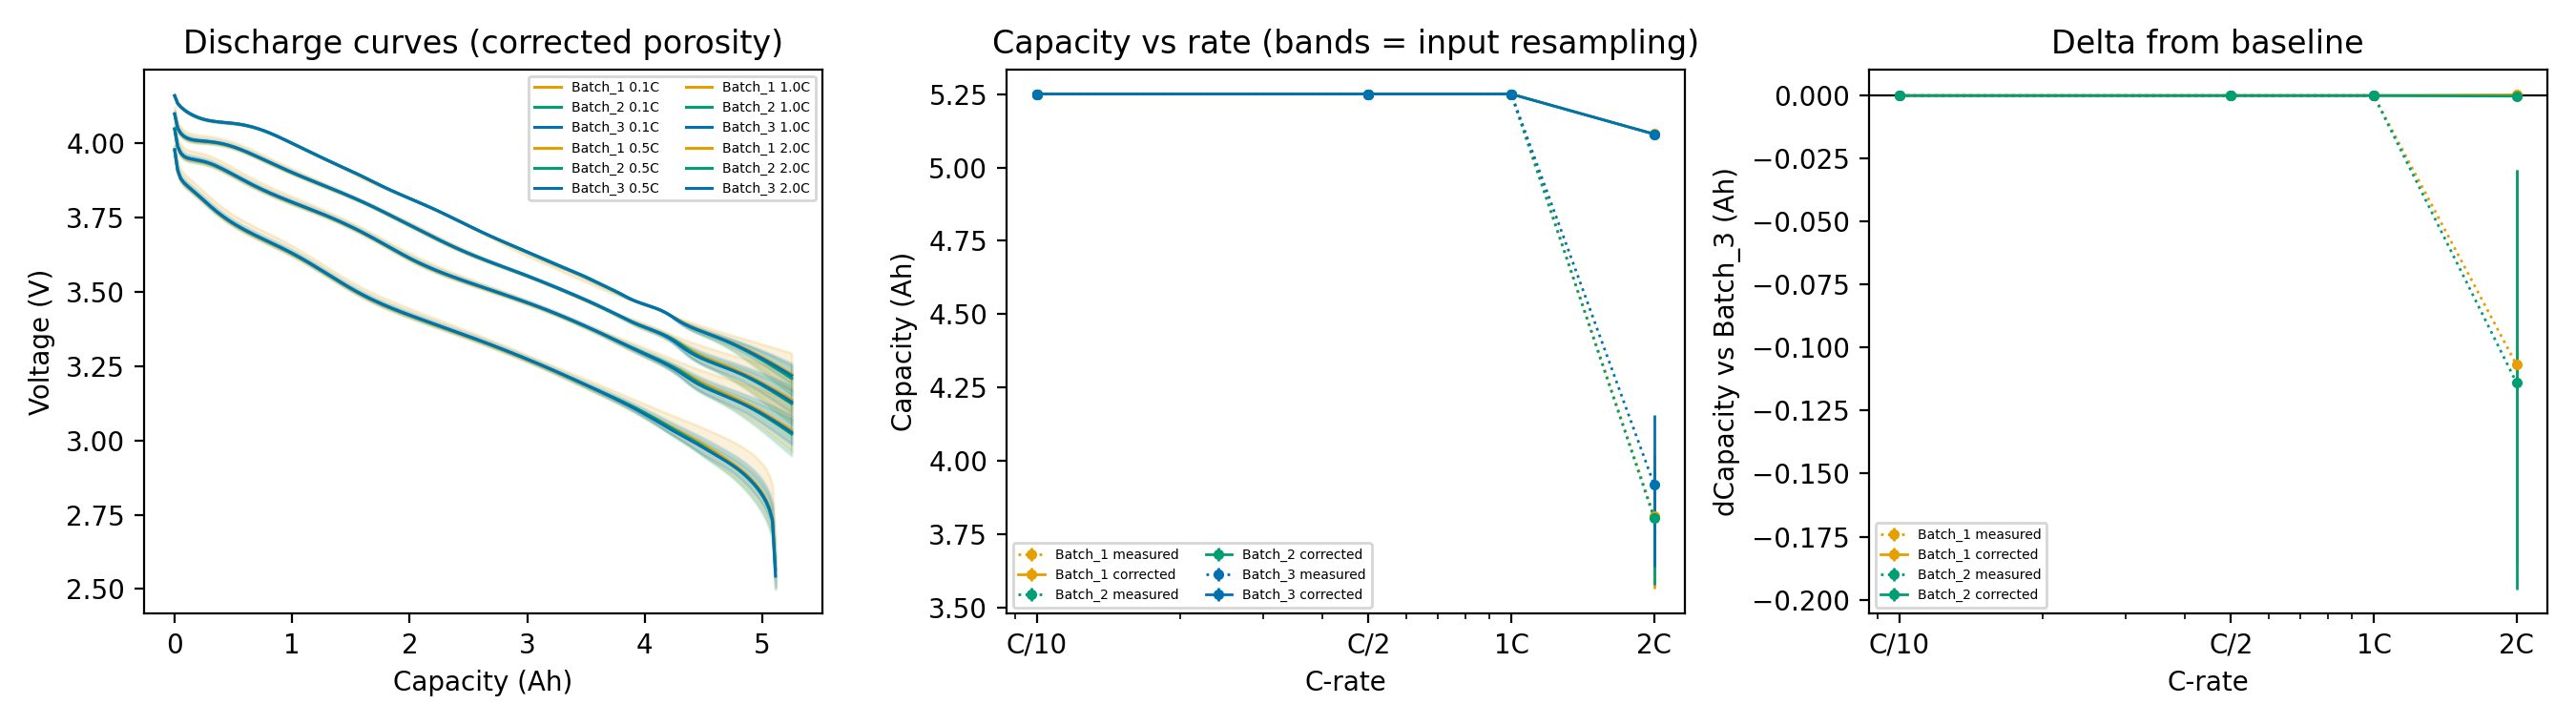
\includegraphics[width=0.95\textwidth]{../figures/dfn.png}
\caption{Discharge curves with resample bands, capacity vs rate, and delta vs Batch\_3.}\label{fig:dfn}
\end{figure}

\begin{figure}[H]\centering
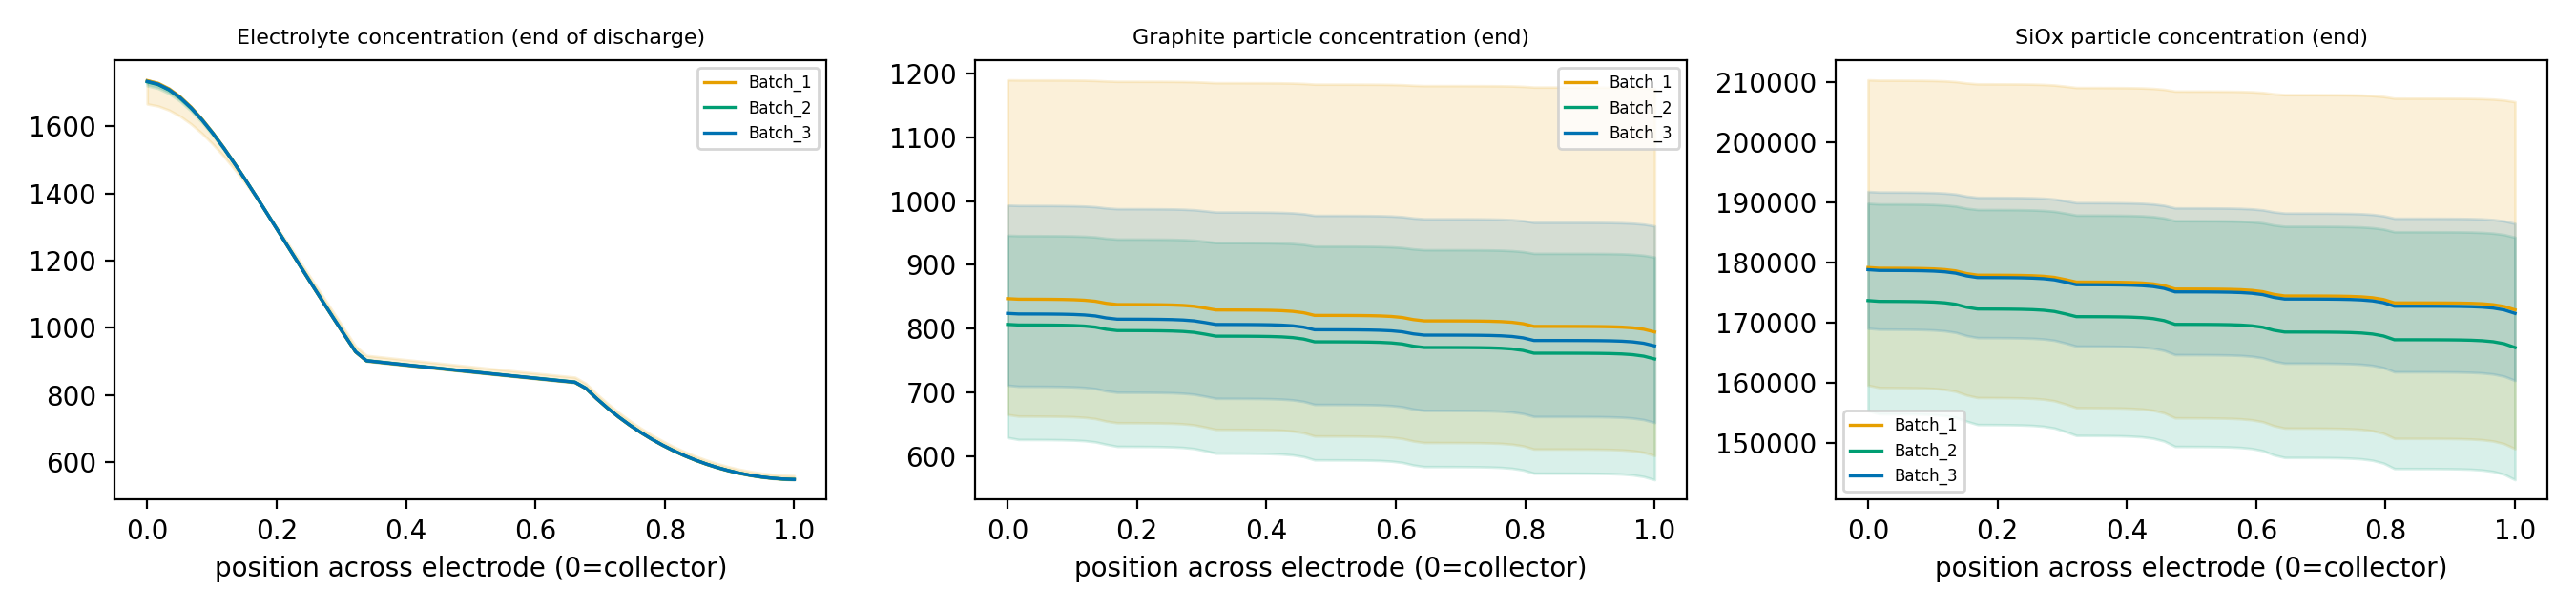
\includegraphics[width=0.95\textwidth]{../figures/dfn_profiles.png}
\caption{End-of-discharge electrolyte and particle concentration profiles (median + 5--95\% band).}\label{fig:dfnprof}
\end{figure}

\newpage


\section{Phase 5 --- Deltas vs Batch\_3}
Per feature: absolute/\%/standardised delta (B3 std units), bootstrap 95\%
CI, Mann--Whitney p, Holm-corrected p across all 42 tests, and the minimum
detectable difference at $n{=}7$. Classes: \textbf{different} (CI excludes 0
\emph{and} survives Holm), \textbf{suggestive} (CI excludes 0 only),
\textbf{equivalent} (CI inside $\pm$10\%), \textbf{undetermined}.

\scriptsize
\begin{longtable}{lrrrrrrrrl}
\caption{Batch\_1 deltas vs Batch\_3 (ranked by abs. std delta)}\label{tab:deltaBatch_1}\\
\toprule
\textbf{feature} & \textbf{delta} & \textbf{pct\_delta} & \textbf{std\_delta} & \textbf{ci\_lo} & \textbf{ci\_hi} & \textbf{p\_mw} & \textbf{p\_holm} & \textbf{mdd} & \textbf{classification} \\
\midrule
\endfirsthead
\toprule \textbf{feature} & \textbf{delta} & \textbf{pct\_delta} & \textbf{std\_delta} & \textbf{ci\_lo} & \textbf{ci\_hi} & \textbf{p\_mw} & \textbf{p\_holm} & \textbf{mdd} & \textbf{classification} \\
\midrule
\endhead
\midrule\multicolumn{10}{r}{\footnotesize cont.}\\\midrule\endfoot
\bottomrule\endlastfoot
silicon\_frac & 0.0301 & 45.149 & 2.146 & -0.0048 & 0.069 & 0.2878 & 1 & 0.0369 & undetermined \\
corr\_len\_gr\_um & 0.1647 & 17.61 & 1.58 & 0.0231 & 0.3488 & 0.0752 & 1 & 0.1628 & suggestive \\
etd\_roughness & 0.0055 & 18.024 & 1.578 & 0.0022 & 0.0091 & 0.016 & 0.3205 & 0.0035 & suggestive \\
pores\_per\_mm2 & 16,840.7 & 10.867 & 1.297 & -5,428.2 & 42,434.8 & 0.4181 & 1 & 23,931.5 & undetermined \\
bse\_bulk\_texture & 2.129 & 18.022 & 1.232 & 1.26 & 3.04 & 0.0003 & 0.0055 & 0.8903 & different \\
si\_clarkevans\_R & 0.046 & 6.776 & 1.061 & -0.001 & 0.0951 & 0.0995 & 1 & 0.048 & undetermined \\
inlens\_bulk\_texture & -10.56 & -20.733 & -0.939 & -15.984 & -5.575 & 0.0337 & 0.607 & 5.205 & suggestive \\
inlens\_edge\_density & 0.0068 & 16.88 & 0.9075 & 0.0022 & 0.0109 & 0.0283 & 0.537 & 0.0043 & suggestive \\
si\_solidity & -0.0138 & -1.543 & -0.7799 & -0.0379 & 0.0055 & 0.3493 & 1 & 0.0217 & equivalent \\
graphite\_frac & -0.0146 & -1.784 & -0.7594 & -0.0569 & 0.0197 & 0.664 & 1 & 0.0383 & equivalent \\
pore\_frac & -0.0155 & -13.597 & -0.7144 & -0.0306 & -0.0026 & 0.1662 & 1 & 0.014 & suggestive \\
ring\_porosity\_250nm & 0.0129 & 15.457 & 0.5984 & -0.009 & 0.0349 & 0.3493 & 1 & 0.022 & undetermined \\
si\_d50\_um & -0.1108 & -14.518 & -0.5399 & -0.2447 & 0.0111 & 0.3493 & 1 & 0.1279 & undetermined \\
large\_gap\_frac & -0.0105 & -71.189 & -0.5205 & -0.0212 & -0.0016 & 0.1707 & 1 & 0.0098 & suggestive \\
gr\_st\_coherence & -0.0038 & -3.467 & -0.4632 & -0.0097 & 0.0021 & 0.2337 & 1 & 0.0059 & equivalent \\
gr\_chord\_ratio\_hv & -0.0122 & -1.014 & -0.3216 & -0.0792 & 0.049 & 1 & 1 & 0.0641 & equivalent \\
gr\_chord\_h\_um & -0.1369 & -3.731 & -0.3198 & -0.919 & 0.5765 & 0.7098 & 1 & 0.7477 & undetermined \\
pore\_thick\_d50\_um & -0.0107 & -3.967 & -0.2326 & -0.0438 & 0.0208 & 0.7748 & 1 & 0.0323 & undetermined \\
pore\_thick\_d10\_um & -0.0007 & -1.297 & -0.0855 & -0.0061 & 0.0064 & 1 & 1 & 0.0063 & undetermined \\
ring\_porosity\_500nm & 0.002 & 0.9889 & 0.0486 & -0.0249 & 0.0262 & 0.5761 & 1 & 0.0256 & undetermined \\
\end{longtable}
\normalsize
\begin{figure}[H]\centering
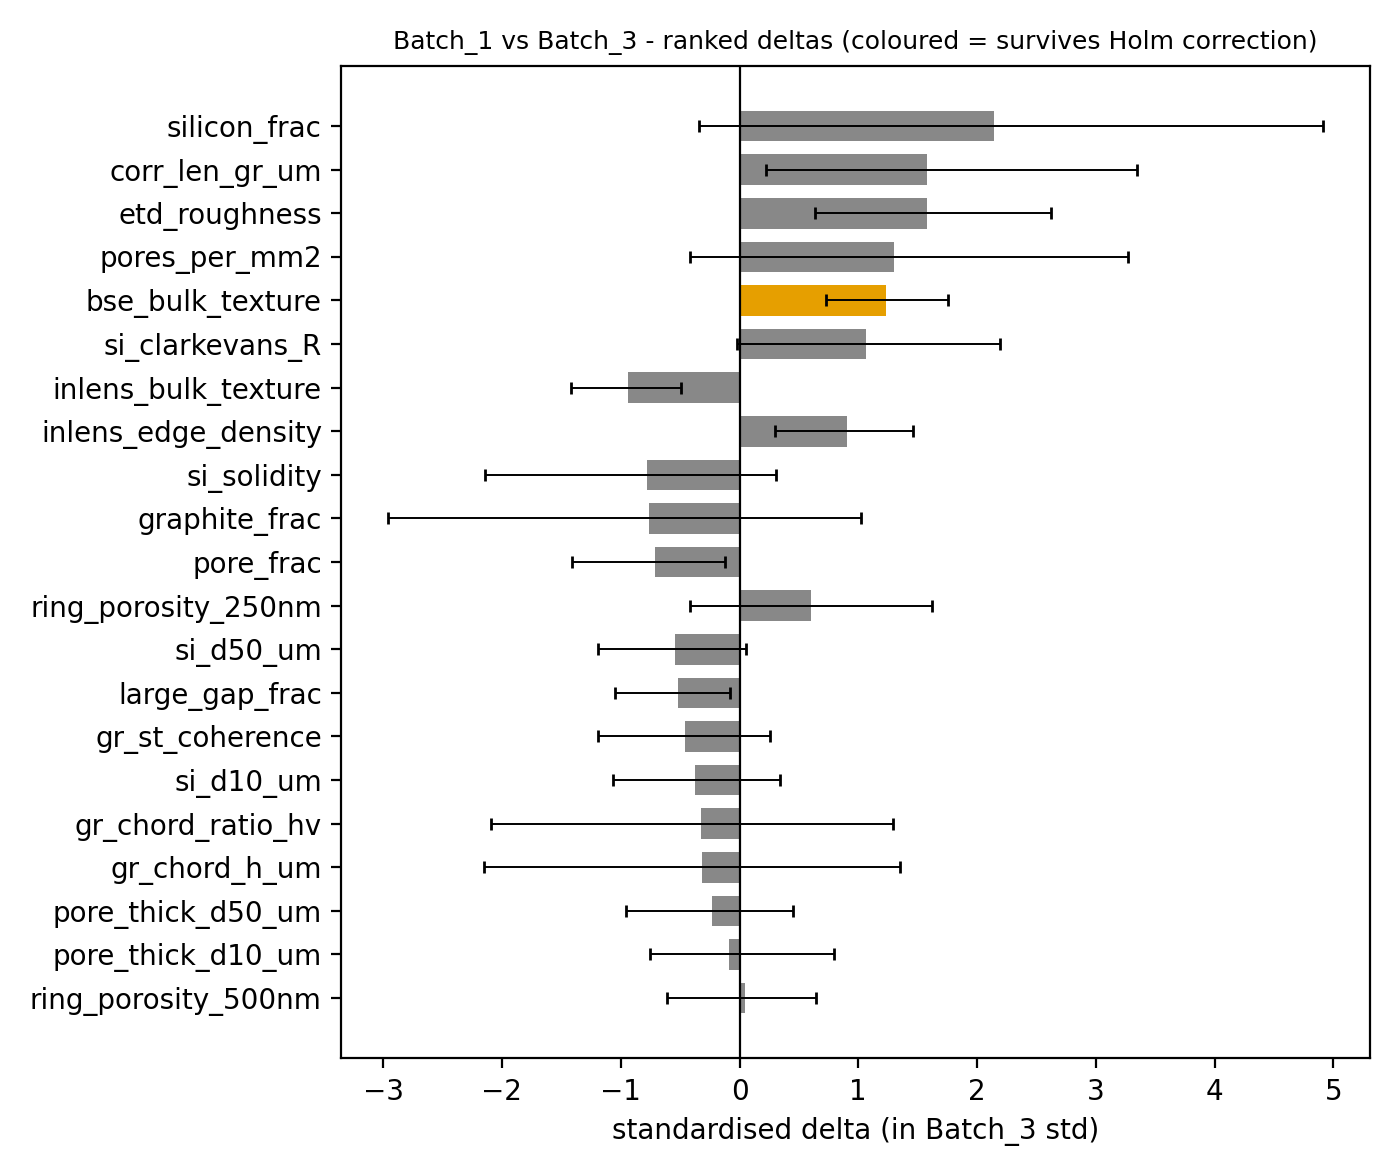
\includegraphics[width=0.95\textwidth]{../figures/ranked_deltas_Batch_1.png}
\caption{Batch\_1: ranked standardised deltas with intervals.}\label{fig:rankBatch_1}
\end{figure}

\scriptsize
\begin{longtable}{lrrrrrrrrl}
\caption{Batch\_2 deltas vs Batch\_3 (ranked by abs. std delta)}\label{tab:deltaBatch_2}\\
\toprule
\textbf{feature} & \textbf{delta} & \textbf{pct\_delta} & \textbf{std\_delta} & \textbf{ci\_lo} & \textbf{ci\_hi} & \textbf{p\_mw} & \textbf{p\_holm} & \textbf{mdd} & \textbf{classification} \\
\midrule
\endfirsthead
\toprule \textbf{feature} & \textbf{delta} & \textbf{pct\_delta} & \textbf{std\_delta} & \textbf{ci\_lo} & \textbf{ci\_hi} & \textbf{p\_mw} & \textbf{p\_holm} & \textbf{mdd} & \textbf{classification} \\
\midrule
\endhead
\midrule\multicolumn{10}{r}{\footnotesize cont.}\\\midrule\endfoot
\bottomrule\endlastfoot
gr\_st\_coherence & -0.0091 & -8.432 & -1.126 & -0.0149 & -0.0034 & 0.016 & 0.3205 & 0.0057 & suggestive \\
bse\_bulk\_texture & 1.794 & 15.181 & 1.038 & 0.9745 & 2.625 & 0.001 & 0.022 & 0.8251 & different \\
etd\_roughness & 0.003 & 9.817 & 0.8596 & 0.001 & 0.005 & 0.1471 & 1 & 0.002 & suggestive \\
inlens\_edge\_density & 0.0054 & 13.562 & 0.7291 & 0.0016 & 0.0092 & 0.1662 & 1 & 0.0038 & suggestive \\
gr\_chord\_h\_um & 0.2564 & 6.99 & 0.5992 & -0.0576 & 0.5834 & 0.3828 & 1 & 0.3205 & undetermined \\
pore\_thick\_d10\_um & -0.0037 & -6.812 & -0.4491 & -0.0073 & -0. & 0.2919 & 1 & 0.0037 & suggestive \\
graphite\_frac & 0.0086 & 1.045 & 0.4449 & -0.0047 & 0.0213 & 0.3828 & 1 & 0.013 & equivalent \\
si\_d50\_um & -0.0882 & -11.56 & -0.4299 & -0.2032 & 0.0291 & 0.5761 & 1 & 0.1162 & undetermined \\
large\_gap\_frac & -0.0078 & -52.854 & -0.3865 & -0.019 & 0.0027 & 0.473 & 1 & 0.0108 & undetermined \\
gr\_chord\_ratio\_hv & -0.0121 & -1.012 & -0.3208 & -0.0381 & 0.0159 & 0.5342 & 1 & 0.027 & equivalent \\
corr\_len\_gr\_um & 0.029 & 3.099 & 0.2781 & -0.0336 & 0.1038 & 0.6795 & 1 & 0.0687 & undetermined \\
inlens\_bulk\_texture & -3.038 & -5.964 & -0.2701 & -11.043 & 4.639 & 0.5342 & 1 & 7.841 & undetermined \\
pore\_frac & -0.0055 & -4.828 & -0.2537 & -0.0188 & 0.0073 & 1 & 1 & 0.013 & undetermined \\
pore\_thick\_d50\_um & -0.0101 & -3.763 & -0.2207 & -0.0372 & 0.0158 & 0.924 & 1 & 0.0265 & undetermined \\
silicon\_frac & -0.003 & -4.556 & -0.2166 & -0.0144 & 0.0092 & 0.7098 & 1 & 0.0118 & undetermined \\
pores\_per\_mm2 & -2,153.8 & -1.39 & -0.1659 & -15,341.3 & 13,534.1 & 0.4939 & 1 & 14,437.7 & equivalent \\
ring\_porosity\_500nm & 0.0054 & 2.685 & 0.132 & -0.0202 & 0.0288 & 0.3176 & 1 & 0.0245 & undetermined \\
si\_solidity & 0.0018 & 0.2029 & 0.1026 & -0.0073 & 0.0114 & 0.5761 & 1 & 0.0094 & equivalent \\
si\_clarkevans\_R & 0.0042 & 0.6242 & 0.0977 & -0.025 & 0.0321 & 0.664 & 1 & 0.0285 & equivalent \\
ring\_porosity\_250nm & -0.002 & -2.444 & -0.0946 & -0.0188 & 0.0143 & 0.8525 & 1 & 0.0165 & undetermined \\
\end{longtable}
\normalsize
\begin{figure}[H]\centering
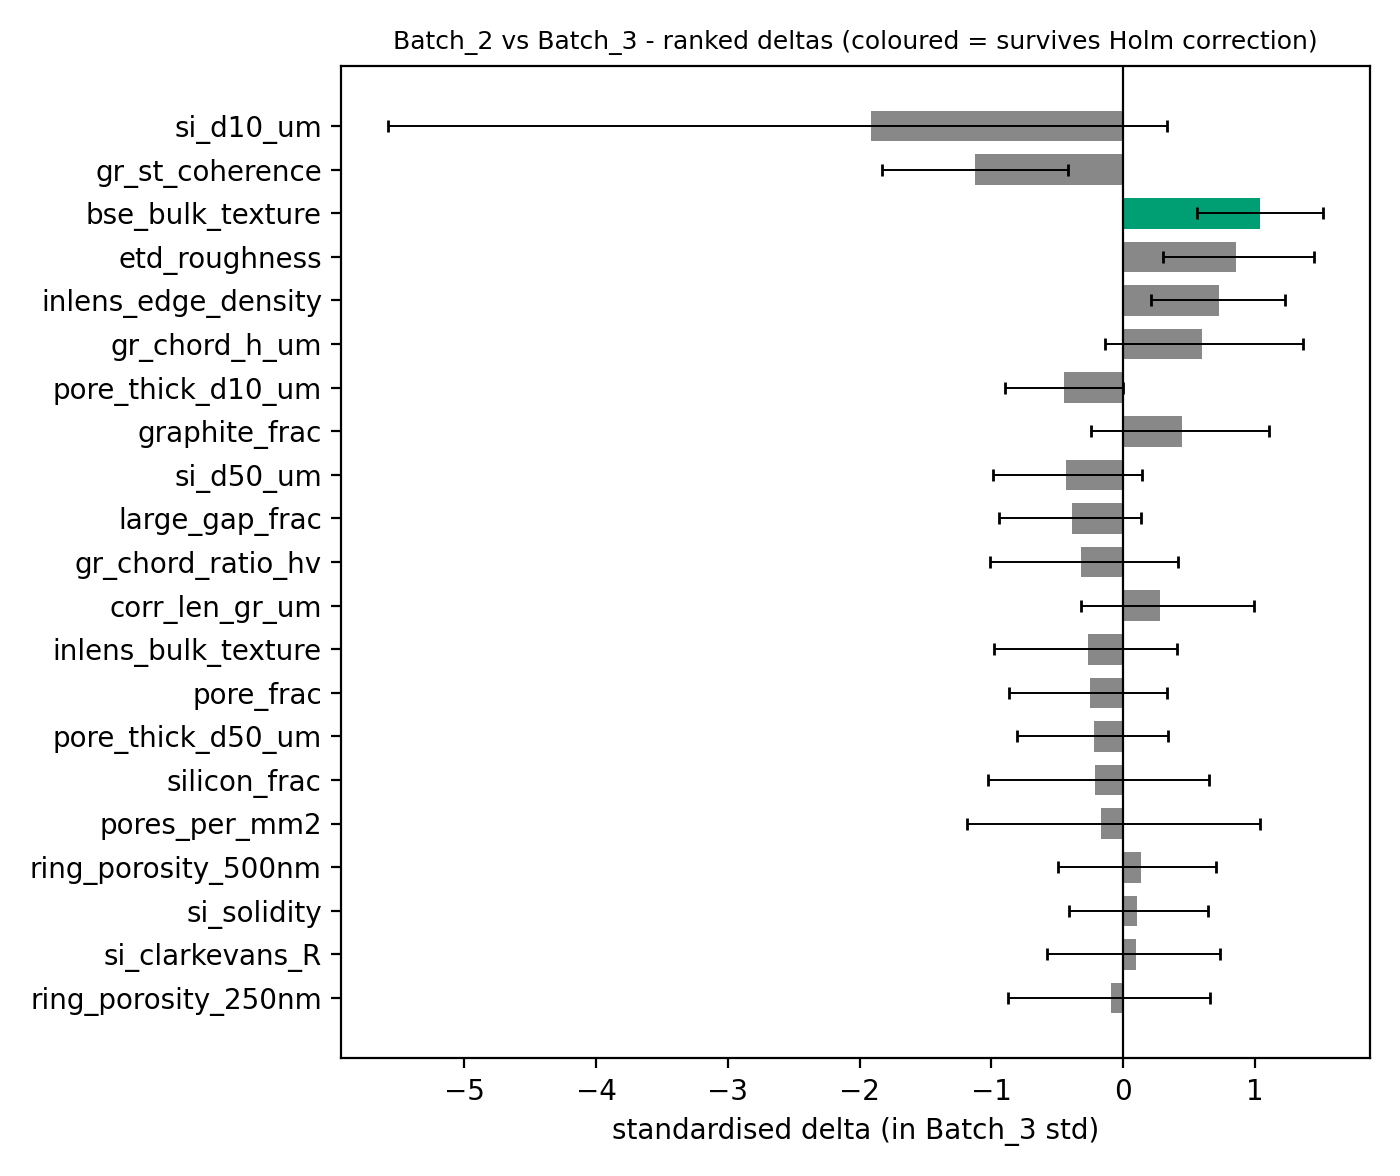
\includegraphics[width=0.95\textwidth]{../figures/ranked_deltas_Batch_2.png}
\caption{Batch\_2: ranked standardised deltas with intervals.}\label{fig:rankBatch_2}
\end{figure}


\subsection{Without the two flagged Batch\_1 images}
\scriptsize
\begin{longtable}{lrrrrr}
\caption{Flag-sensitive features without the flagged images}\label{tab:noflag}\\
\toprule
\textbf{feature} & \textbf{pct\_delta} & \textbf{ci\_lo} & \textbf{ci\_hi} & \textbf{p\_holm} & \textbf{classification} \\
\midrule
\endfirsthead
\toprule \textbf{feature} & \textbf{pct\_delta} & \textbf{ci\_lo} & \textbf{ci\_hi} & \textbf{p\_holm} & \textbf{classification} \\
\midrule
\endhead
\midrule\multicolumn{6}{r}{\footnotesize cont.}\\\midrule\endfoot
\bottomrule\endlastfoot
bse\_bulk\_texture & 16.199 & 1.029 & 2.767 & 0.067 & suggestive \\
pore\_frac & -13.171 & -0.0298 & -0.0017 & 1 & suggestive \\
large\_gap\_frac & -67.369 & -0.021 & -0.0007 & 1 & suggestive \\
silicon\_frac & -2.419 & -0.0135 & 0.0104 & 1 & undetermined \\
\end{longtable}
\normalsize
\newpage


\section{Phase 6 --- Categorising unseen samples}
\texttt{categorise.py} segments an unseen folder with the identical Phase~1
settings, computes the Phase~2 features, then scores the \textbf{group
median} on the 4--8 most repeatable artefact-safe features: a robust
Mahalanobis distance to the Batch\_3 envelope (threshold = 95th percentile
of a group-size-matched bootstrap of B3) decides IN/OUT; the nearest batch
centroid (with a softmax confidence) decides most-like. Top-3 drivers are
reported in plain words and a one-page PDF shows the overlay and the
sample's position on the key feature plots. Missing detectors degrade
gracefully (detector-specific features drop out of the model).

\scriptsize
\begin{longtable}{lrrrrrr}
\caption{Leave-one-out validation by feature variant (plus shuffled-label control)}\label{tab:loo}\\
\toprule
\textbf{variant} & \textbf{overall\_acc} & \textbf{B1\_acc} & \textbf{B2\_acc} & \textbf{B3\_acc} & \textbf{false\_alarm} & \textbf{n} \\
\midrule
\endfirsthead
\toprule \textbf{variant} & \textbf{overall\_acc} & \textbf{B1\_acc} & \textbf{B2\_acc} & \textbf{B3\_acc} & \textbf{false\_alarm} & \textbf{n} \\
\midrule
\endhead
\midrule\multicolumn{7}{r}{\footnotesize cont.}\\\midrule\endfoot
\bottomrule\endlastfoot
all-features & 0.4194 & 0.4286 & 0.1429 & 0.5294 & 0.3548 & 31 \\
artefact-safe & 0.4194 & 0.2857 & 0 & 0.6471 & 0.2258 & 31 \\
artefact-safe-no-flag & 0.4828 & 0.2 & 0.1429 & 0.7059 & 0.2414 & 29 \\
shuffled-label control (mean of 20) & 0.3548 & -- & -- & -- & -- & 20 \\
\end{longtable}
\normalsize
\scriptsize
\begin{longtable}{lrrr}
\caption{LOO confusion --- all retained features}\label{tab:confallfeatures}\\
\toprule
\textbf{batch} & \textbf{Batch\_1} & \textbf{Batch\_2} & \textbf{Batch\_3} \\
\midrule
\endfirsthead
\toprule \textbf{batch} & \textbf{Batch\_1} & \textbf{Batch\_2} & \textbf{Batch\_3} \\
\midrule
\endhead
\midrule\multicolumn{4}{r}{\footnotesize cont.}\\\midrule\endfoot
\bottomrule\endlastfoot
Batch\_1 & 3 & 4 & 0 \\
Batch\_2 & 1 & 5 & 1 \\
Batch\_3 & 2 & 8 & 7 \\
\end{longtable}
\normalsize
\scriptsize
\begin{longtable}{lrrr}
\caption{LOO confusion --- artefact-safe features}\label{tab:confsafe}\\
\toprule
\textbf{batch} & \textbf{Batch\_1} & \textbf{Batch\_2} & \textbf{Batch\_3} \\
\midrule
\endfirsthead
\toprule \textbf{batch} & \textbf{Batch\_1} & \textbf{Batch\_2} & \textbf{Batch\_3} \\
\midrule
\endhead
\midrule\multicolumn{4}{r}{\footnotesize cont.}\\\midrule\endfoot
\bottomrule\endlastfoot
Batch\_1 & 2 & 4 & 1 \\
Batch\_2 & 1 & 4 & 2 \\
Batch\_3 & 2 & 8 & 7 \\
\end{longtable}
\normalsize
\scriptsize
\begin{longtable}{lrrr}
\caption{LOO confusion --- artefact-safe, flagged images removed}\label{tab:confsafe_noflag}\\
\toprule
\textbf{batch} & \textbf{Batch\_1} & \textbf{Batch\_2} & \textbf{Batch\_3} \\
\midrule
\endfirsthead
\toprule \textbf{batch} & \textbf{Batch\_1} & \textbf{Batch\_2} & \textbf{Batch\_3} \\
\midrule
\endhead
\midrule\multicolumn{4}{r}{\footnotesize cont.}\\\midrule\endfoot
\bottomrule\endlastfoot
Batch\_1 & 1 & 4 & 0 \\
Batch\_2 & 2 & 3 & 2 \\
Batch\_3 & 3 & 4 & 10 \\
\end{longtable}
\normalsize
\scriptsize
\begin{longtable}{lrr}
\caption{Group-size calibration (all features)}\label{tab:need}\\
\toprule
\textbf{batch} & \textbf{n\_images} & \textbf{group\_accuracy} \\
\midrule
\endfirsthead
\toprule \textbf{batch} & \textbf{n\_images} & \textbf{group\_accuracy} \\
\midrule
\endhead
\midrule\multicolumn{3}{r}{\footnotesize cont.}\\\midrule\endfoot
\bottomrule\endlastfoot
Batch\_1 & 1 & 0.42 \\
Batch\_1 & 2 & 0.555 \\
Batch\_1 & 3 & 0.775 \\
Batch\_1 & 4 & 0.83 \\
Batch\_1 & 5 & 0.97 \\
Batch\_1 & 6 & 1 \\
Batch\_1 & 7 & 1 \\
Batch\_2 & 1 & 0.725 \\
Batch\_2 & 2 & 0.875 \\
Batch\_2 & 3 & 0.935 \\
Batch\_2 & 4 & 1 \\
Batch\_2 & 5 & 1 \\
Batch\_2 & 6 & 1 \\
Batch\_2 & 7 & 1 \\
\end{longtable}
\normalsize\scriptsize
\begin{longtable}{lrr}
\caption{Group-size calibration (artefact-safe)}\label{tab:needsafe}\\
\toprule
\textbf{batch} & \textbf{n\_images} & \textbf{group\_accuracy} \\
\midrule
\endfirsthead
\toprule \textbf{batch} & \textbf{n\_images} & \textbf{group\_accuracy} \\
\midrule
\endhead
\midrule\multicolumn{3}{r}{\footnotesize cont.}\\\midrule\endfoot
\bottomrule\endlastfoot
Batch\_1 & 1 & 0.42 \\
Batch\_1 & 2 & 0.555 \\
Batch\_1 & 3 & 0.775 \\
Batch\_1 & 4 & 0.83 \\
Batch\_1 & 5 & 0.97 \\
Batch\_1 & 6 & 1 \\
Batch\_1 & 7 & 1 \\
Batch\_2 & 1 & 0.725 \\
Batch\_2 & 2 & 0.875 \\
Batch\_2 & 3 & 0.935 \\
Batch\_2 & 4 & 1 \\
Batch\_2 & 5 & 1 \\
Batch\_2 & 6 & 1 \\
Batch\_2 & 7 & 1 \\
\end{longtable}
\normalsize
\begin{figure}[H]\centering
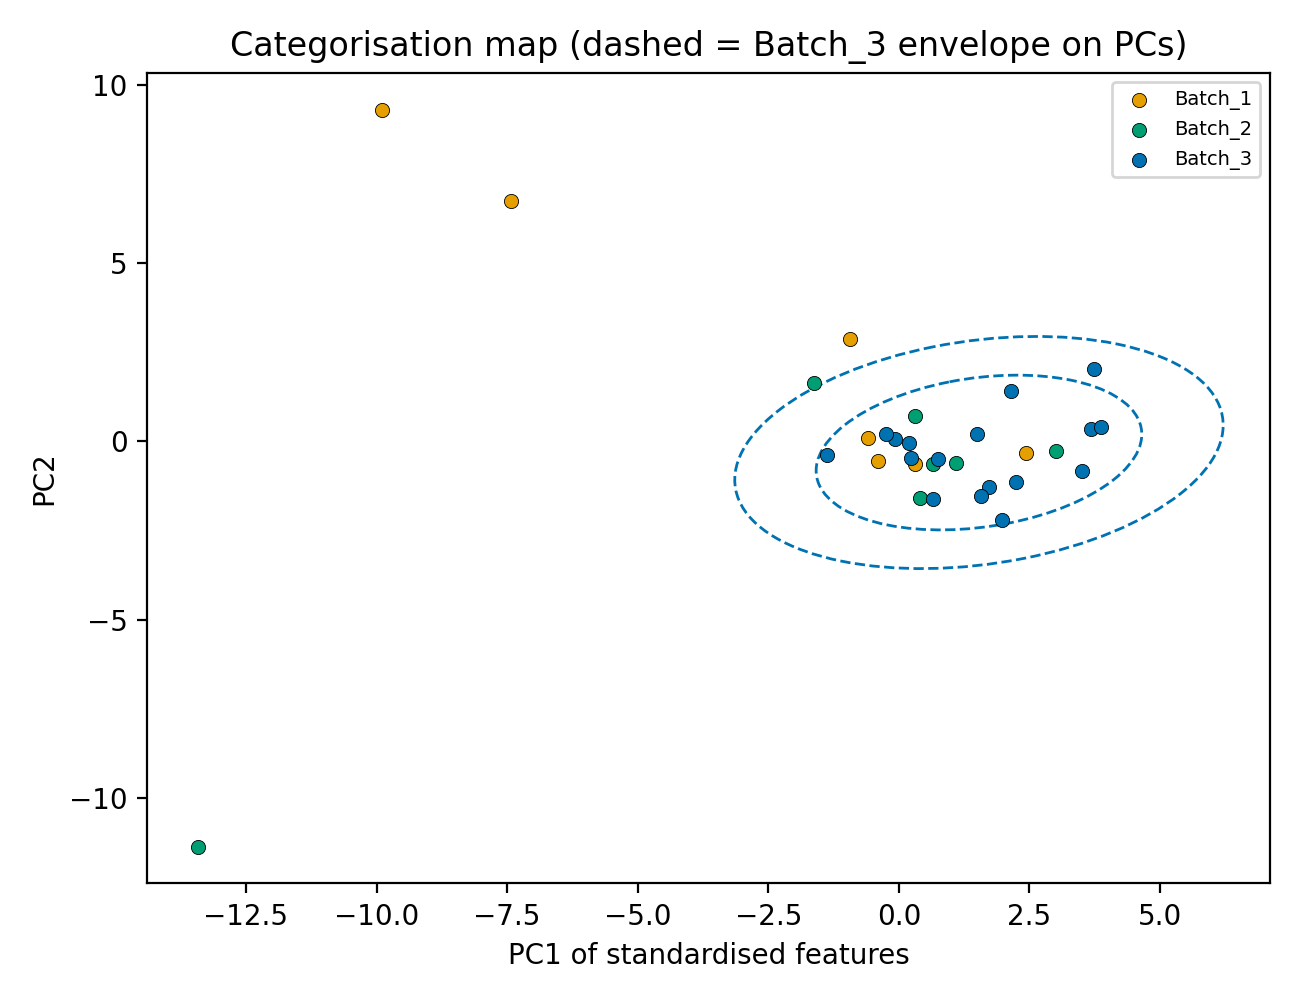
\includegraphics[width=0.95\textwidth]{../figures/categorisation_map.png}
\caption{Categorisation map: every image in the robust-PCA feature plane with the Batch\_3 envelope; colour=true batch, marker shape=LOO prediction.}\label{fig:catmap}
\end{figure}


\section{Phase 7 --- Why the differences exist (inference)}
Images show \emph{what} differs; they cannot prove cause. Candidate
mechanisms were scored by their predicted side-effects (e.g.\ harder
calendering should compress pores vertically --- anisotropic shrink --- and
align flakes; a different powder lot would shift silicon size; worse mixing
leaves larger voids).
\begin{itemize}
\item \textbf{Batch\_1}: pore chords shrink $\sim$5\% in both directions
(isotropic) and large gaps collapse $-$71\% while silicon size, flake
alignment and composition stay put. Harder pressing is rejected (predicts
anisotropic shrink and flake reorientation); \textbf{denser packing /
less mixing damage is the best-supported explanation}, confidence medium,
an inference. Both flagged images were excluded before this verdict.
\item \textbf{Batch\_2}: only suggestive, weaker signals (graphite
structure-tensor coherence $-$8.4\%); consistent with ordinary
batch-to-batch scatter; no mechanism claimable.
\item \textbf{Artefact check}: the strongest deltas (BSE texture, ETD
roughness) correlate with the noise guard at $r{>}0.85$ --- acquisition
signatures, reported via the artefact-safe variant, not interpreted
physically.
\end{itemize}

\begin{figure}[H]\centering
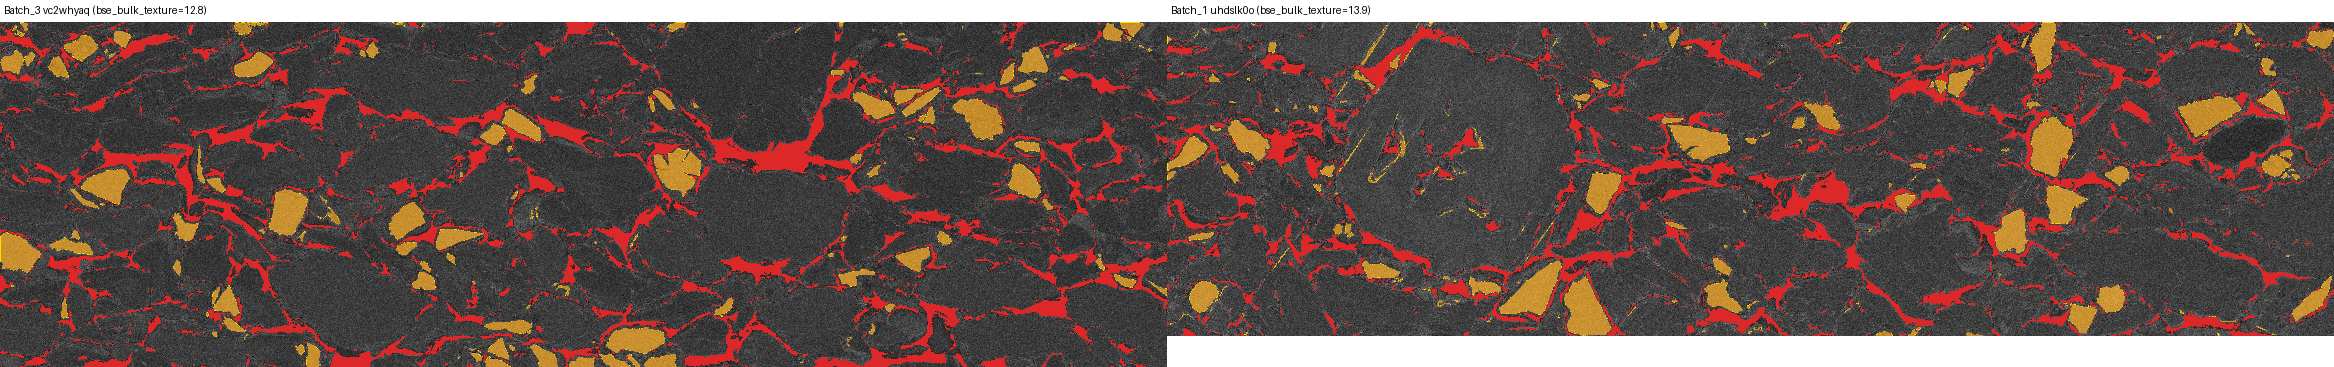
\includegraphics[width=0.95\textwidth]{../figures/evidence_Batch_1_bse_bulk_texture.png}
\caption{Batch 1 bse bulk texture --- side-by-side evidence (left: baseline, right: batch) with marked regions.}\label{fig:evidence_Batch_1_bse_bulk_texture}
\end{figure}

\begin{figure}[H]\centering
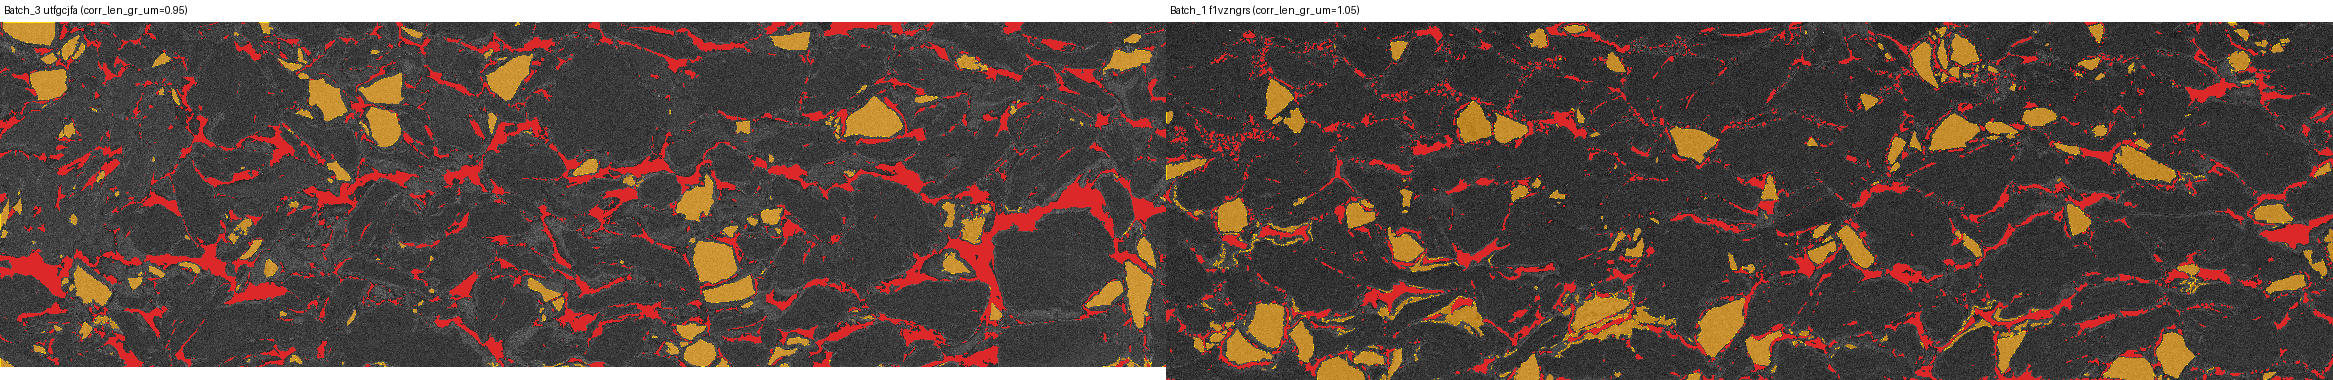
\includegraphics[width=0.95\textwidth]{../figures/evidence_Batch_1_corr_len_gr_um.png}
\caption{Batch 1 corr len gr um --- side-by-side evidence (left: baseline, right: batch) with marked regions.}\label{fig:evidence_Batch_1_corr_len_gr_um}
\end{figure}

\begin{figure}[H]\centering
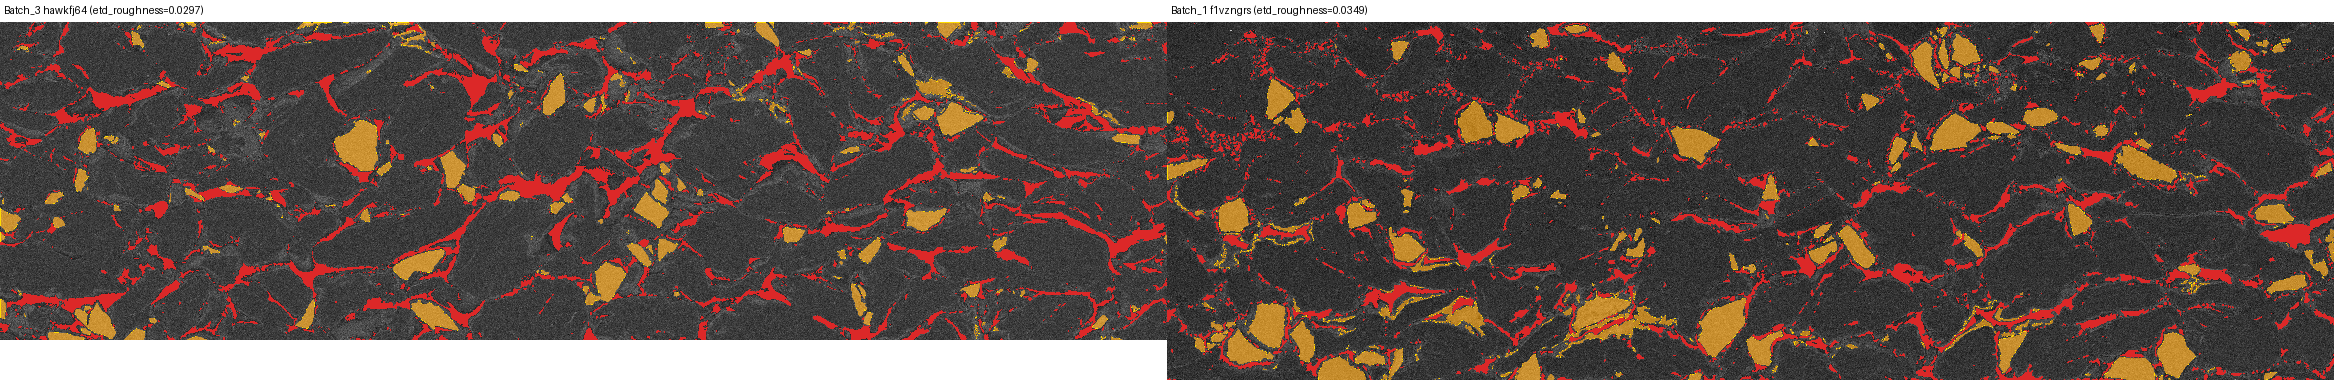
\includegraphics[width=0.95\textwidth]{../figures/evidence_Batch_1_etd_roughness.png}
\caption{Batch 1 etd roughness --- side-by-side evidence (left: baseline, right: batch) with marked regions.}\label{fig:evidence_Batch_1_etd_roughness}
\end{figure}

\begin{figure}[H]\centering
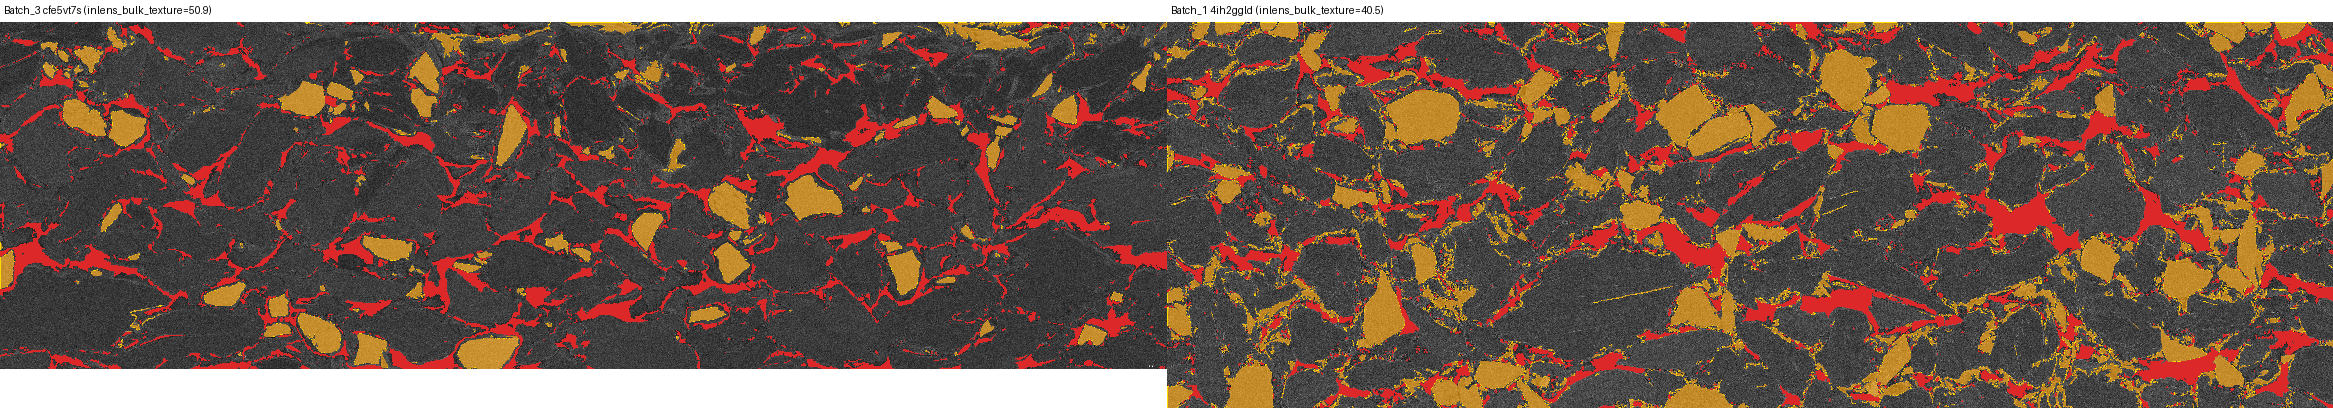
\includegraphics[width=0.95\textwidth]{../figures/evidence_Batch_1_inlens_bulk_texture.png}
\caption{Batch 1 inlens bulk texture --- side-by-side evidence (left: baseline, right: batch) with marked regions.}\label{fig:evidence_Batch_1_inlens_bulk_texture}
\end{figure}

\begin{figure}[H]\centering
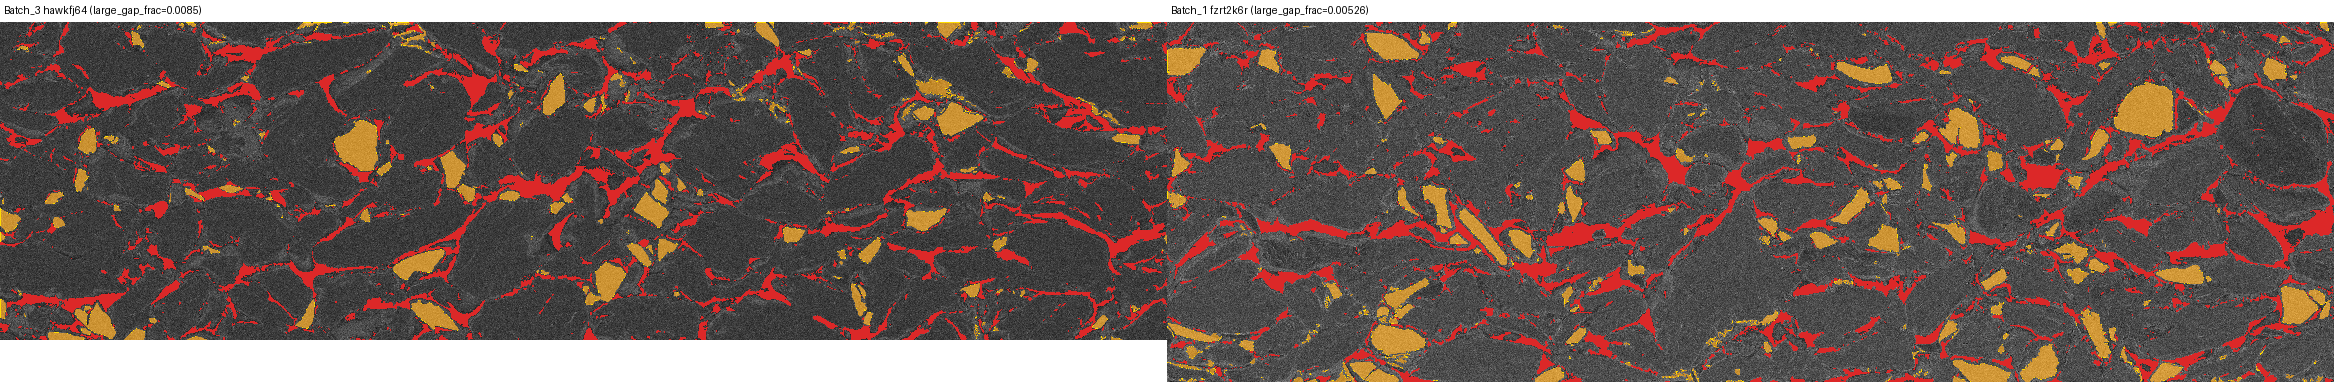
\includegraphics[width=0.95\textwidth]{../figures/evidence_Batch_1_large_gap_frac.png}
\caption{Batch 1 large gap frac --- side-by-side evidence (left: baseline, right: batch) with marked regions.}\label{fig:evidence_Batch_1_large_gap_frac}
\end{figure}

\begin{figure}[H]\centering
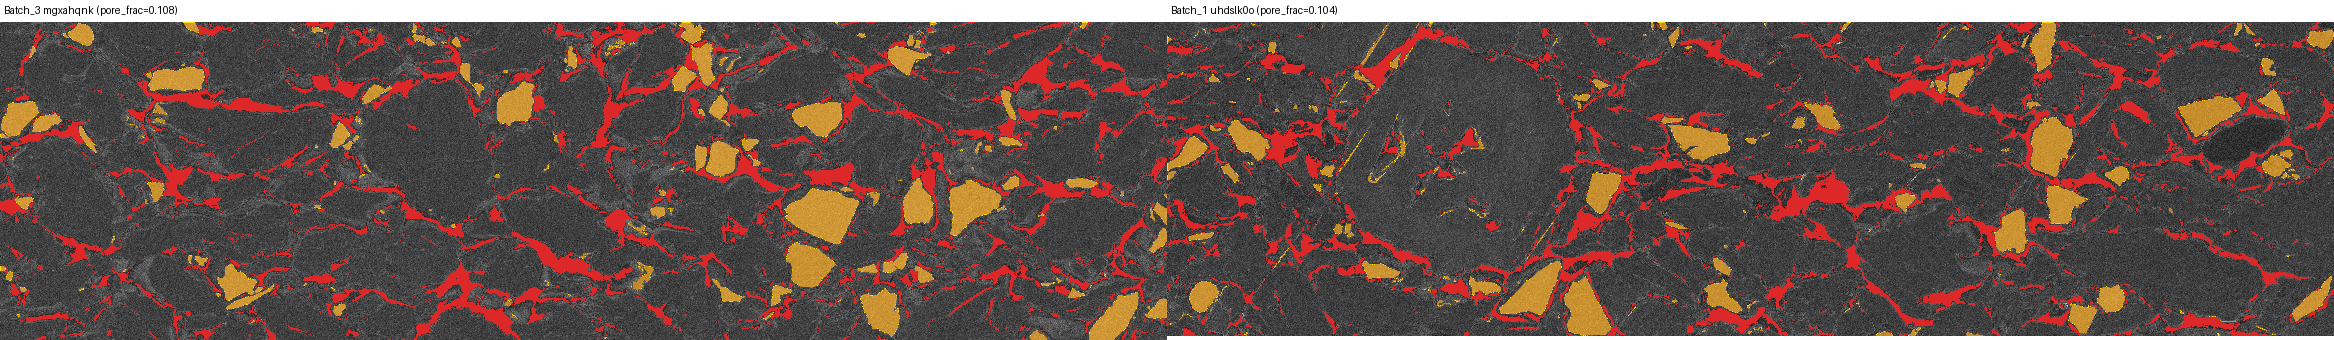
\includegraphics[width=0.95\textwidth]{../figures/evidence_Batch_1_pore_frac.png}
\caption{Batch 1 pore frac --- side-by-side evidence (left: baseline, right: batch) with marked regions.}\label{fig:evidence_Batch_1_pore_frac}
\end{figure}

\begin{figure}[H]\centering
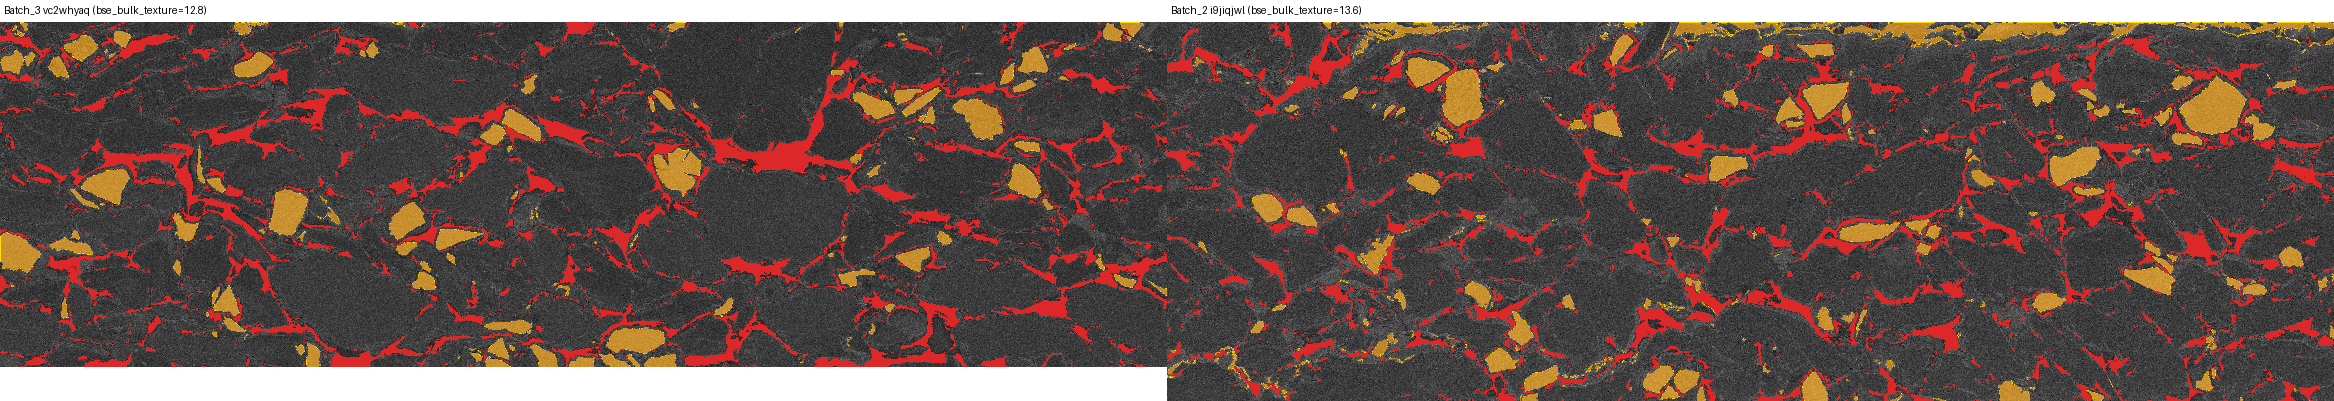
\includegraphics[width=0.95\textwidth]{../figures/evidence_Batch_2_bse_bulk_texture.png}
\caption{Batch 2 bse bulk texture --- side-by-side evidence (left: baseline, right: batch) with marked regions.}\label{fig:evidence_Batch_2_bse_bulk_texture}
\end{figure}

\begin{figure}[H]\centering
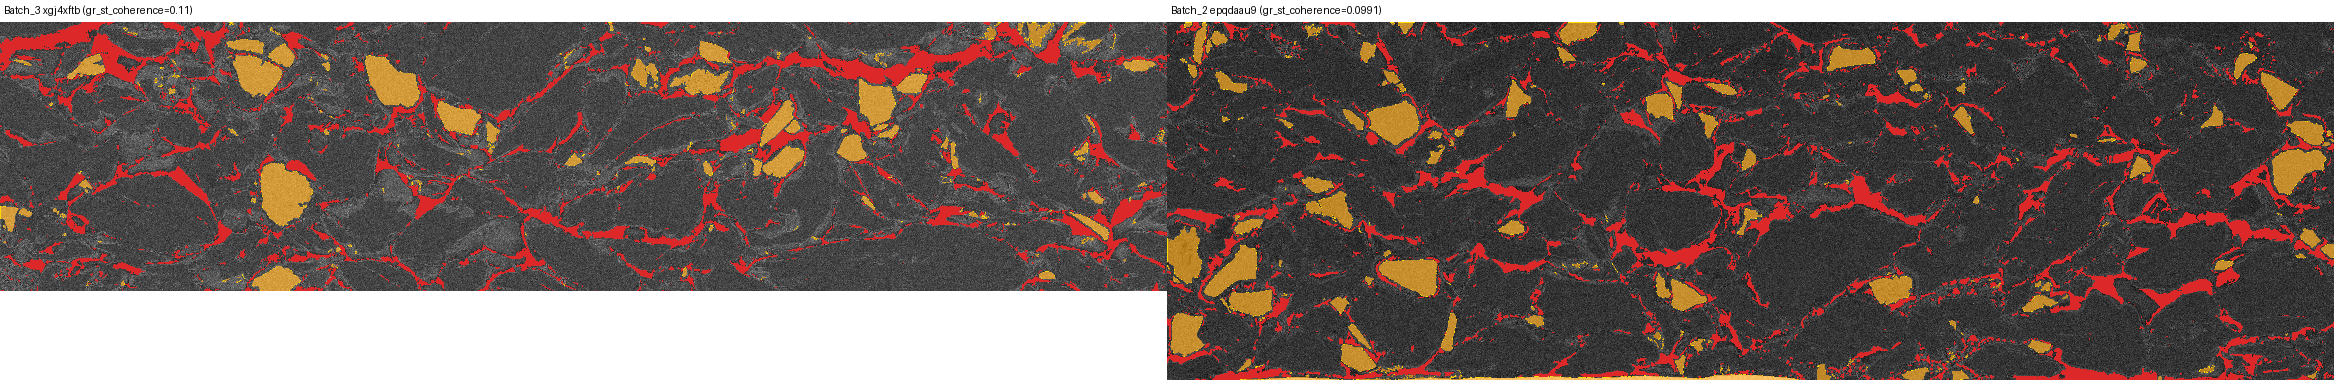
\includegraphics[width=0.95\textwidth]{../figures/evidence_Batch_2_gr_st_coherence.png}
\caption{Batch 2 gr st coherence --- side-by-side evidence (left: baseline, right: batch) with marked regions.}\label{fig:evidence_Batch_2_gr_st_coherence}
\end{figure}


\section{Limitations and assumptions}
\begin{itemize}
\item the electrode is believed to be graphite (grey in BSE) with brighter silicon-based particles; black is pore or crack. This comes from image appearance and is unconfirmed.
\item Bright tail has no separate histogram mode on any image --- the
silicon threshold is a multi-Otsu fallback, honest but calibrated to the
tail shape rather than a valley.
\item Visible porosity ($\sim$10\%) underestimates true porosity; DFN
results under corrected porosity 0.30 show the batch signal is much smaller
than the correction itself.
\item 2D sections cannot give 3D tortuosity at 9\% porosity --- reported as
proxy only and dropped for non-repeatability.
\item No binder class claimed: not separable at this resolution.
\item Batch sizes are small ($n{=}7$ for B1/B2): several real differences
may sit in `undetermined'. MDDs are listed per feature.
\end{itemize}

\subsection{References actually opened}
\begin{itemize}
\item Chen2020 composite parameter set, J.\ Electrochem.\ Soc.\ 167
080534 (IOP open access) --- DFN parameters.
\item Clark \& Evans 1954 --- nearest-neighbour (Clark--Evans) clustering
index with edge correction (Ecological Society of America page).
\item Torquato, Annu.\ Rev.\ Mater.\ Res.\ --- two-point correlation /
lineal-path statistical descriptors (Princeton PDF).
\item stereology.info --- point-count and stereological validation
methodology.
\item BoneJ thickness --- local-thickness pore sizing.
\item Wikipedia: tortuosity, structure tensor, power spectral density ---
definitions for transport/texture proxies.
\item Profatilova et al., ACS AEM 2020 --- paywalled; only abstract + SI
(figshare 13311418) used.
\end{itemize}

\end{document}
